\documentclass[final,hyperref={pdfpagelabels=false}]{beamer}
\usepackage{grffile}
\mode<presentation>{\usetheme{I6pd2}}
\usepackage[english]{babel}
\usepackage[spanish]{babel}
\usepackage[latin1]{inputenc}
\usepackage{amsmath,amsthm, amssymb, latexsym}
\usepackage{tikz}
\usetikzlibrary{shapes.geometric, arrows,backgrounds,fit}
\usepackage{booktabs}
\usepackage{caption}
\captionsetup{justification={justified}}
\usepackage[square,numbers]{natbib}
\usepackage{ragged2e}
\tikzstyle{arrow} = [thick,line width=0.8mm,->,>=stealth]
\usepackage{hyperref}

%\usepackage{times}\usefonttheme{professionalfonts}  % obsolete
%\usefonttheme[onlymath]{serif}
\boldmath
\usepackage[orientation=portrait,size=a0,scale=1.4,debug]{beamerposter}
% change list indention level
% \setdefaultleftmargin{3em}{}{}{}{}{}


%\usepackage{snapshot} % will write a .dep file with all dependencies, allows for easy bundling

\usepackage{array,booktabs,tabularx}
\newcolumntype{Z}{>{\centering\arraybackslash}X} % centered tabularx columns
\newcommand{\pphantom}{\textcolor{ta3aluminium}} % phantom introduces a vertical space in p formatted table columns??!!
\setbeamercolor{background canvas}{bg=lightgray}
\setbeamercolor*{block body}{bg=white, fg=black}
\listfiles

%%%%%%%%%%%%%%%%%%%%%%%%%%%%%%%%%%%%%%%%%%%%%%%%%%%%%%%%%%%%%%%%%%%%%%%%%%%%%%%%%%%%%%

\graphicspath{{figures/}}
 
\vspace{0.5cm}\title{\huge Exploring variational autoencoders potential to classify single-cell RNA-seq data}
\author{Bego\~na Bolos Sierra$^{1}$, Felix Pacheco Pastor$^1$, Paula Rodriguez$^1$, Laura Sans-Comerma$^1$ and Ole Winther$^{2,3}$}
\institute[Department]{\small 1 DTU Bioinformatics, Technical University of Denmark; 2 The Bioinformatics Centre, Department of Biology, University of Copenhagen, 3 DTU Compute, Technical University of Denmark}
\date[December 10th, 2020]{December 10th, 2020}

%%%%%%%%%%%%%%%%%%%%%%%%%%%%%%%%%%%%%%%%%%%%%%%%%%%%%%%%%%%%%%%%%%%%%%%%%%%%%%%%%%%%%%
\newlength{\columnheight}
\setlength{\columnheight}{105cm}

\begin{document}

\begin{frame}
 \begin{columns}
% ---------------------------------------------------------%
% Set up  COLUMN 1
% ---------------------------------------------------------%
 \begin{column}{.49\paperwidth}
 \begin{beamercolorbox}[center,wd=\textwidth]{postercolumn}
 \begin{minipage}[T]{.99\textwidth}  % tweaks the width, makes a new \textwidth
 \parbox[t][\columnheight]{\textwidth}{ % must be some better way to set the the height, width and textwidth simultaneously
                                                            % Since all columns are the same length, it is all nice and tidy.  You have to get the height empirically

% ---------------------------------------------------------%
% set up block  INTRODUCTION
% ---------------------------------------------------------%
\begin{block}{Introduction}
 \begin{columns}
 \begin{column}{1\textwidth}
    \centering
    \begin{minipage}[t]{0.97\textwidth}
    
    \vspace{0.5cm}
    \small{
    
    Gene expression levels of individual cells are measured by \textbf{single-cell RNA sequencing} (scRNA-seq).  This procedure generates large amounts of count data, which is characterized for being highly dimensional and sparse. Therefore, current analysis approaches require intensive pre-processing steps.
    
    \vspace{0.5cm} Deep generative models, such as \textbf{variational auto-encoders} (VAE) can be used to analyze scRNA-seq data, generating latent representations which capture most variability of gene expression levels. The library \textbf{scVAE} applies VAE on raw scRNA-seq data, omitting all pre-processing steps and producing a latent representation useful for downstream analyses \cite{gronbech2020}.

    
    \vspace{0.5cm}In this study, the potential of generative models such as scVAE will be evaluated on a cell type classification problem. To do so, a latent representation of the data will be trained by a Feed Forward Neural Network (FFNN) to classify the cell types. The classification will be compared to a FFNN used on sparse raw data and a sub composition by performing Principal Component Analysis (PCA). The data set used corresponds to 10x-PBMC-68k \cite{zheng2017a}.
    \vspace{0.5cm}
    }
    \end{minipage} 
    %\hspace{0cm}


\end{column}
 \end{columns}
 \end{block}
 \vfill


% ---------------------------------------------------------%
% set up block  DATA
% ---------------------------------------------------------%

 \begin{block}{Hypothesis and validation steps}
 \begin{columns}
 \begin{column}{1\textwidth}
\centering
\begin{minipage}[t]{0.97\textwidth}
\justifying
\vspace{0.5cm}
\small{\textbf{Hypothesis:} scVAE latent representation improves cell type classification in comparison with the direct use of sparse count data and/or other dimensionality reduction strategies.}
\vspace{1.2cm}

\textbf{Steps to validate hypothesis:}
\vspace{0.3cm}

\begin{itemize}

\item{\small{Compute 16 scVAE models with different hidden units and latent dimensions.}}
\vspace{0.1cm}
\item{\small{Evaluation and selection of best models, based on ELBO and Rand Index.}}
\vspace{0.1cm}
\item{\small{Perform PCA to raw count data.}}
\vspace{0.1cm}
\item{\small{Build a FFNN to classify cell type.
}}
\vspace{0.1cm}
\item{\small{Compare classification accuracy of the FFNN trained on:}}
\begin{enumerate}
\item{\small{Raw data.}}
\item{\small{scVAE latent representation.}}
\item{\small{PCA components.}}
\end{enumerate}
\vspace{0.1cm}
\end{itemize}

\end{minipage} 
%\end{minipage} \hspace{1cm} \begin{minipage}[t]{.5\textwidth}

\vspace{1cm}

          
\end{column}
\end{columns}
\vskip-1ex
\end{block}
\vfill


% ---------------------------------------------------------%
% set up block  WORKFLOW
% ---------------------------------------------------------%

 \begin{block}{Workflow}
 \begin{columns}
 \begin{column}{1\textwidth}

\centering
\begin{minipage}[t]{0.96\textwidth}
			
\hspace{0.5cm} 
\begin{figure}
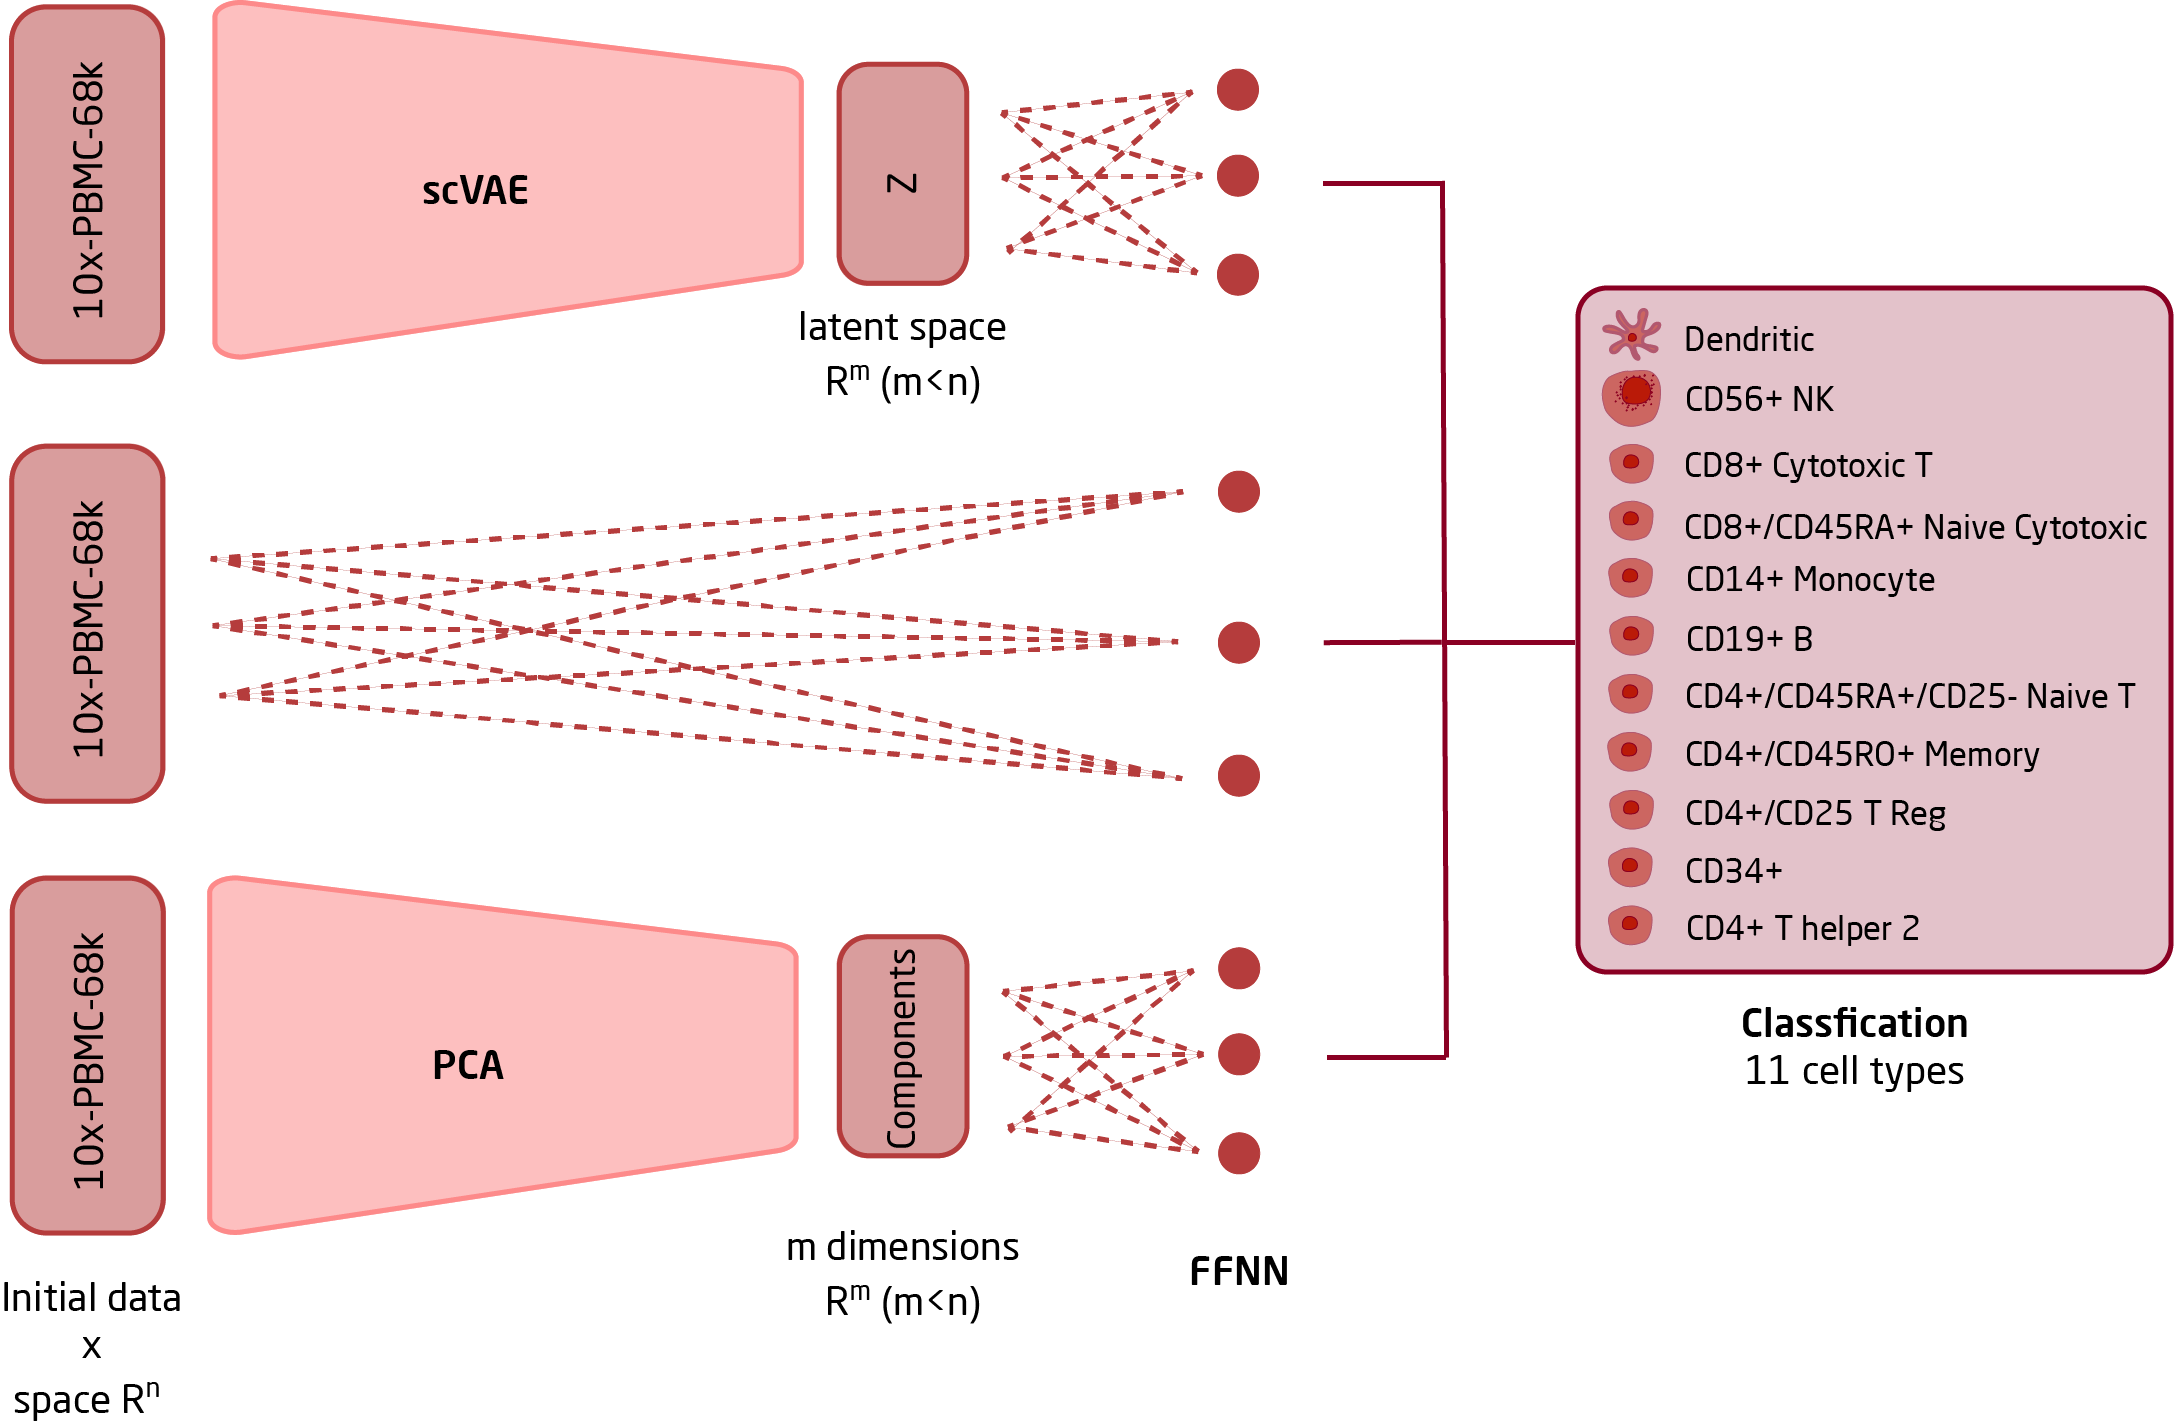
\includegraphics[clip,width=0.95\textwidth]{latex poster/figure_color.png}
 \caption{Overview of the workflow}
 \end{figure}  	


\end{minipage}

\vspace{0.5cm}

					
                  
\end{column}
\end{columns}
\vskip-1ex
\end{block}

\vfill
% ---------------------------------------------------------%
% data ? 
% ---------------------------------------------------------%

\begin{block}{scVAE model performance}
\begin{columns}
\begin{column}{1\textwidth}

    \centering
    \begin{minipage}[t]{0.96\textwidth}
    %\justifying
    %\small{We see in the figure \ref{figure:elbo}, that around epoch 50 the ELBO values reach a plateau phase.}			

    \begin{columns}
    \begin{column}{0.50\textwidth} 
    \centering

    \begin{figure}
        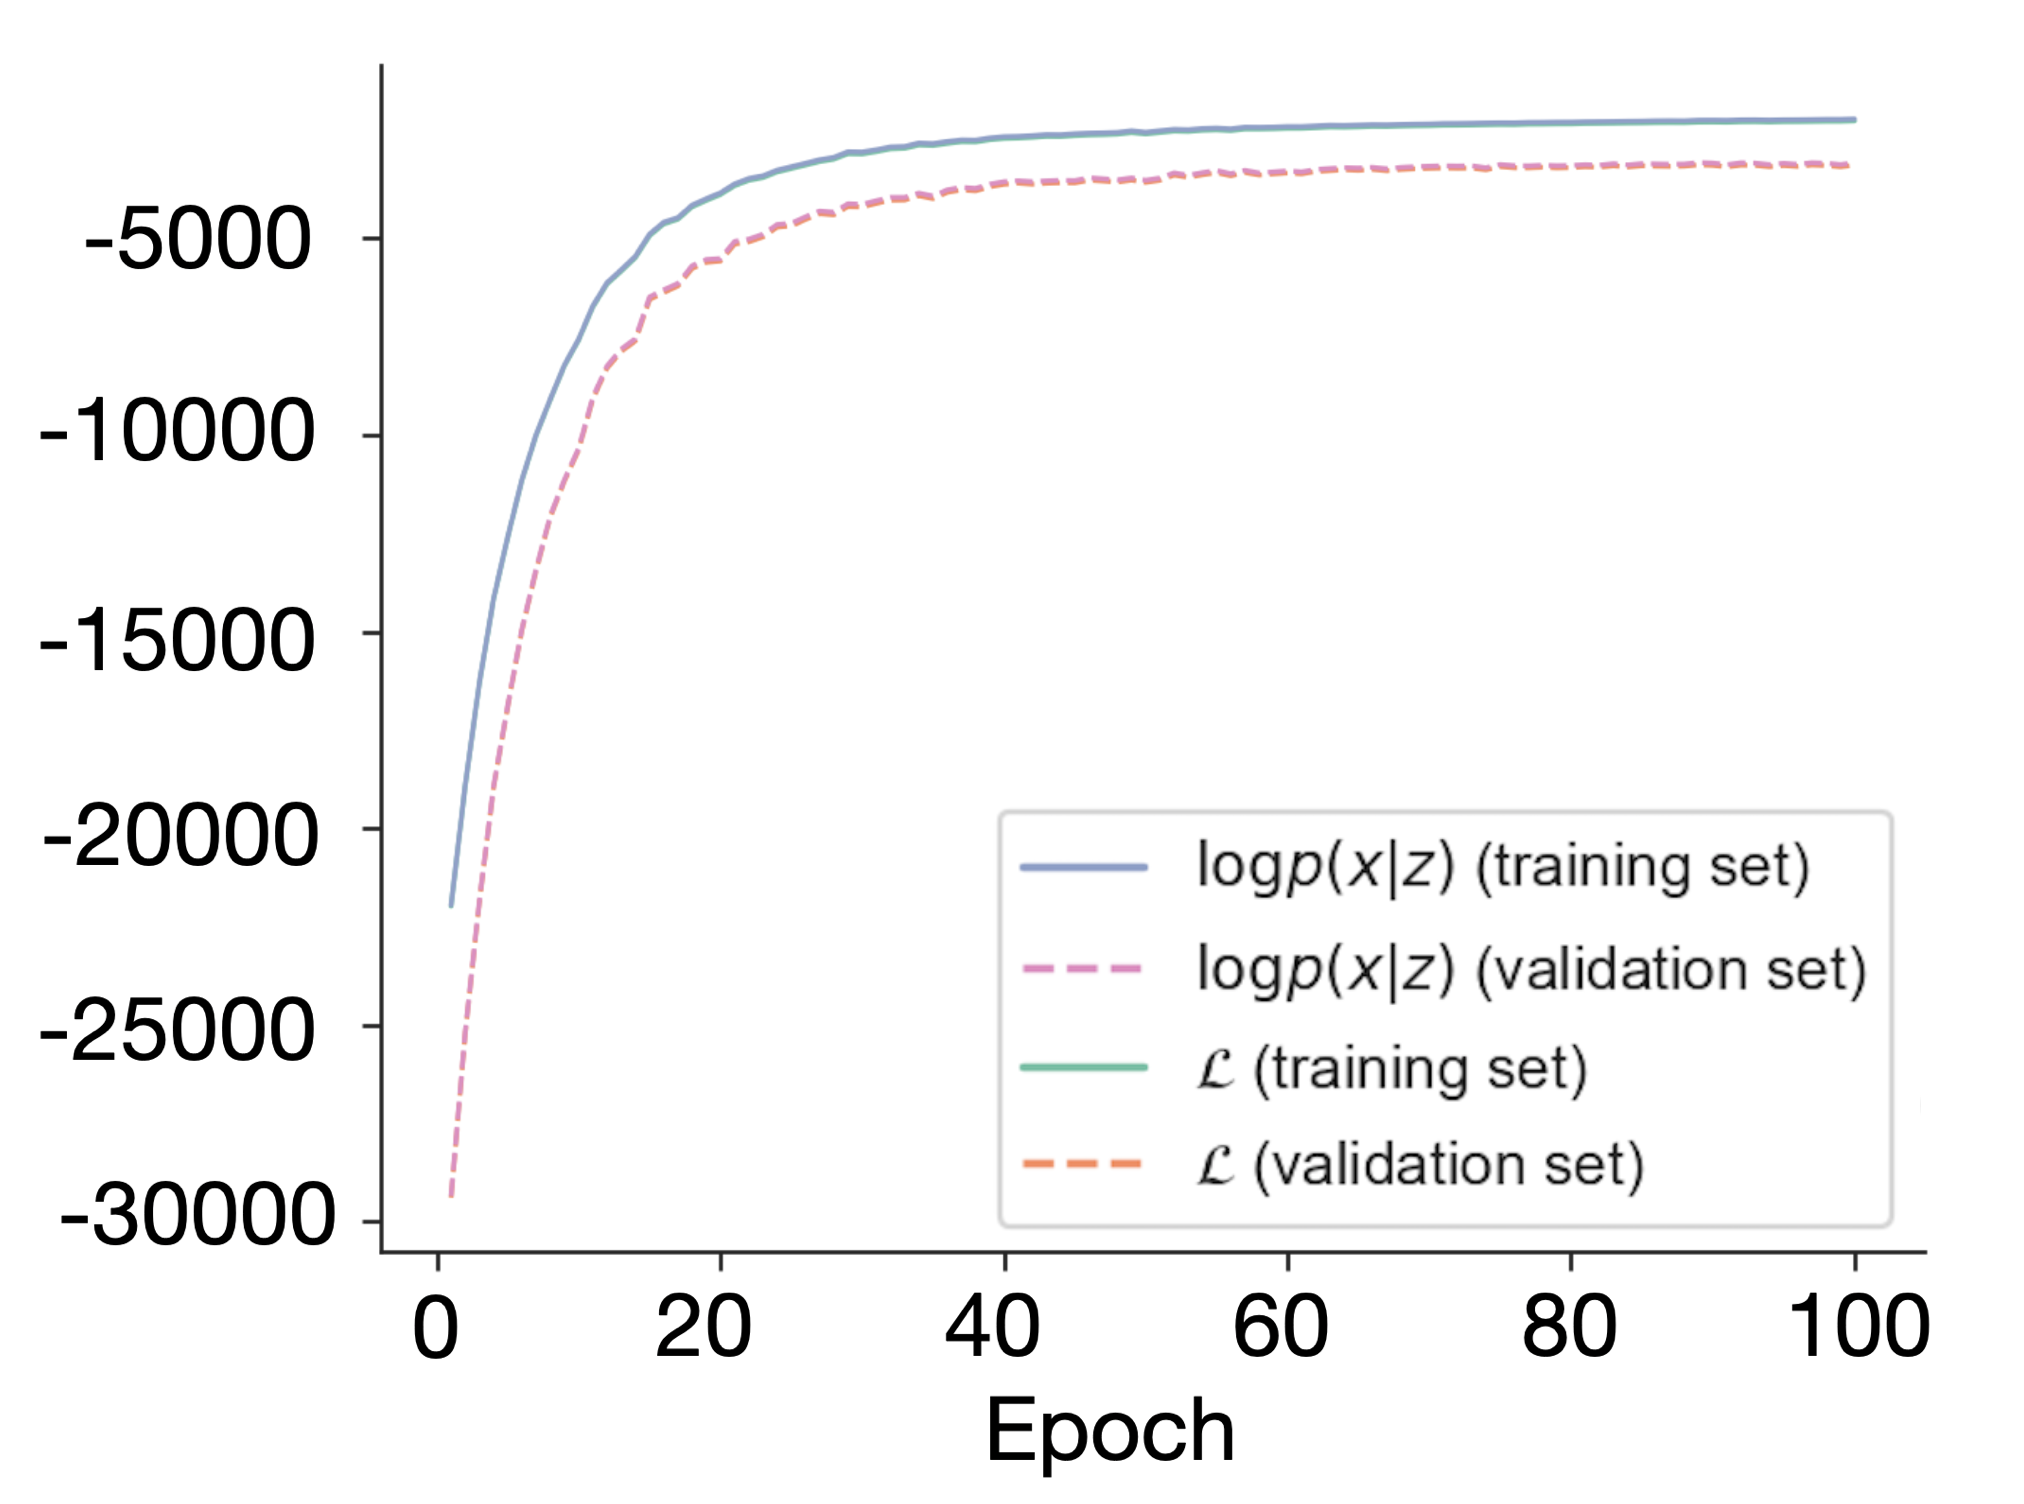
\includegraphics[width=1\textwidth]{latex poster/elbo_training.png}
        \centering
        \caption{ELBO values across epochs. \\ Model hyperparameters: Z=100, H=500}
         \label{figure:elbo}
    \end{figure}  

    \begin{table}[h]
        \small
        \caption{\small{Statistics of top-performance models.\label{table:models}}}
        \centering
        \begin{tabular}{cccc}
            \hline
            Z & H & ELBO    & Rand Index \\ \hline
            10                                          & 250          & -4420.9 & 0.118      \\ 
            25                                          & 500          & -2704.2 & 0.110      \\ 
            50                                          & 250          & -2868.5 & 0.111      \\ 
            \textbf{100}                                         & \textbf{500}          & \textbf{-2387.5} & \textbf{0.106}      \\ 
            \hline
        \end{tabular}
    \end{table}

    \end{column}

    \begin{column}{0.50\textwidth}
        
        \begin{figure}
            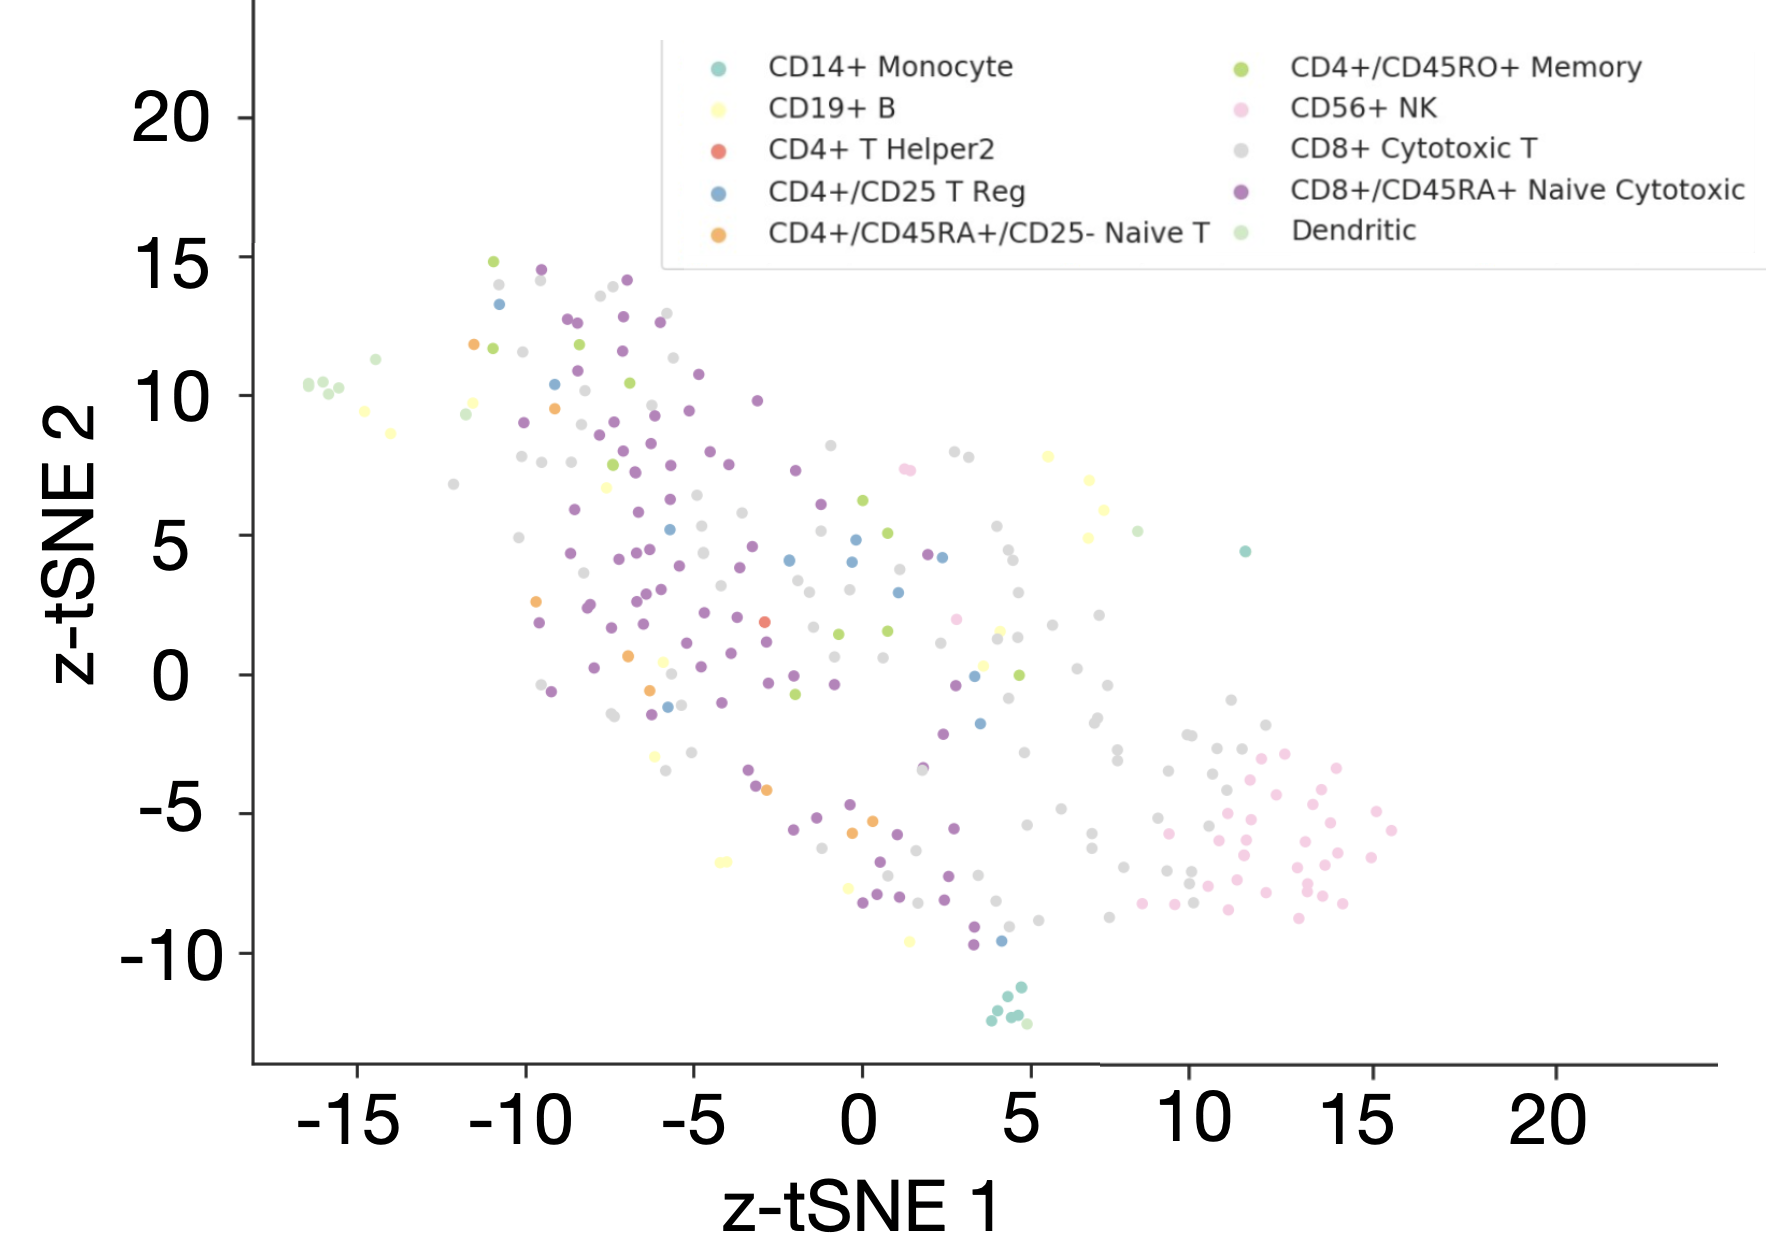
\includegraphics[width=0.99\textwidth]{latex poster/tsne.png}
            \centering
            \caption{tSNE values of latent representation. \\ Model hyperparameters: Z=100, H=500}
             \label{figure:elbo}
        \end{figure} 
        \vspace{1cm}
        \justifying{\\
        \small{\textit{Z:} Latent space dimensions \\
        \textit{H:} Number of hidden units\\
        \textit{Rand index:} Clustering quality.\\
        \textit{ELBO:} Evidence Lower Bound.
        }
        }
        \vspace{2cm}
    \end{column}
\end{columns}
\vspace{0.5cm}

\end{minipage}

\end{column}
\end{columns}
\vskip-1ex
\end{block}
\vfill

% ---------------------------------------------------------%
% set up block REFERENCES
% ---------------------------------------------------------%
}
\end{minipage}
\end{beamercolorbox}
\end{column}
% ---------------------------------------------------------%
% end the COLUMN 1
% ---------------------------------------------------------%
 

% ---------------------------------------------------------%
% Set up COLUMN 2
% ---------------------------------------------------------%
    
\begin{column}{.49\paperwidth}
\begin{beamercolorbox}[center,wd=\textwidth]{postercolumn}
\begin{minipage}[T]{.99\textwidth} % tweaks the width, makes a new \textwidth
\parbox[t][\columnheight]{\textwidth}{ % must be some better way to set the the height, width and textwidth simultaneously
            											% Since all columns are the same length, it is all nice and tidy.  You have to get the height empirically
            
% ---------------------------------------------------------%
% set up block RESULTS + DISCUSSION
% ---------------------------------------------------------%

\begin{block}{Cell type classification with feed-forward neural network}
\begin{columns}
% -- COL 1

\begin{column}{0.49\textwidth}
\centering
%\vspace{2.5cm}

\begin{minipage}[t]{.95\textwidth}
\vspace{0.5cm}
\begin{figure}
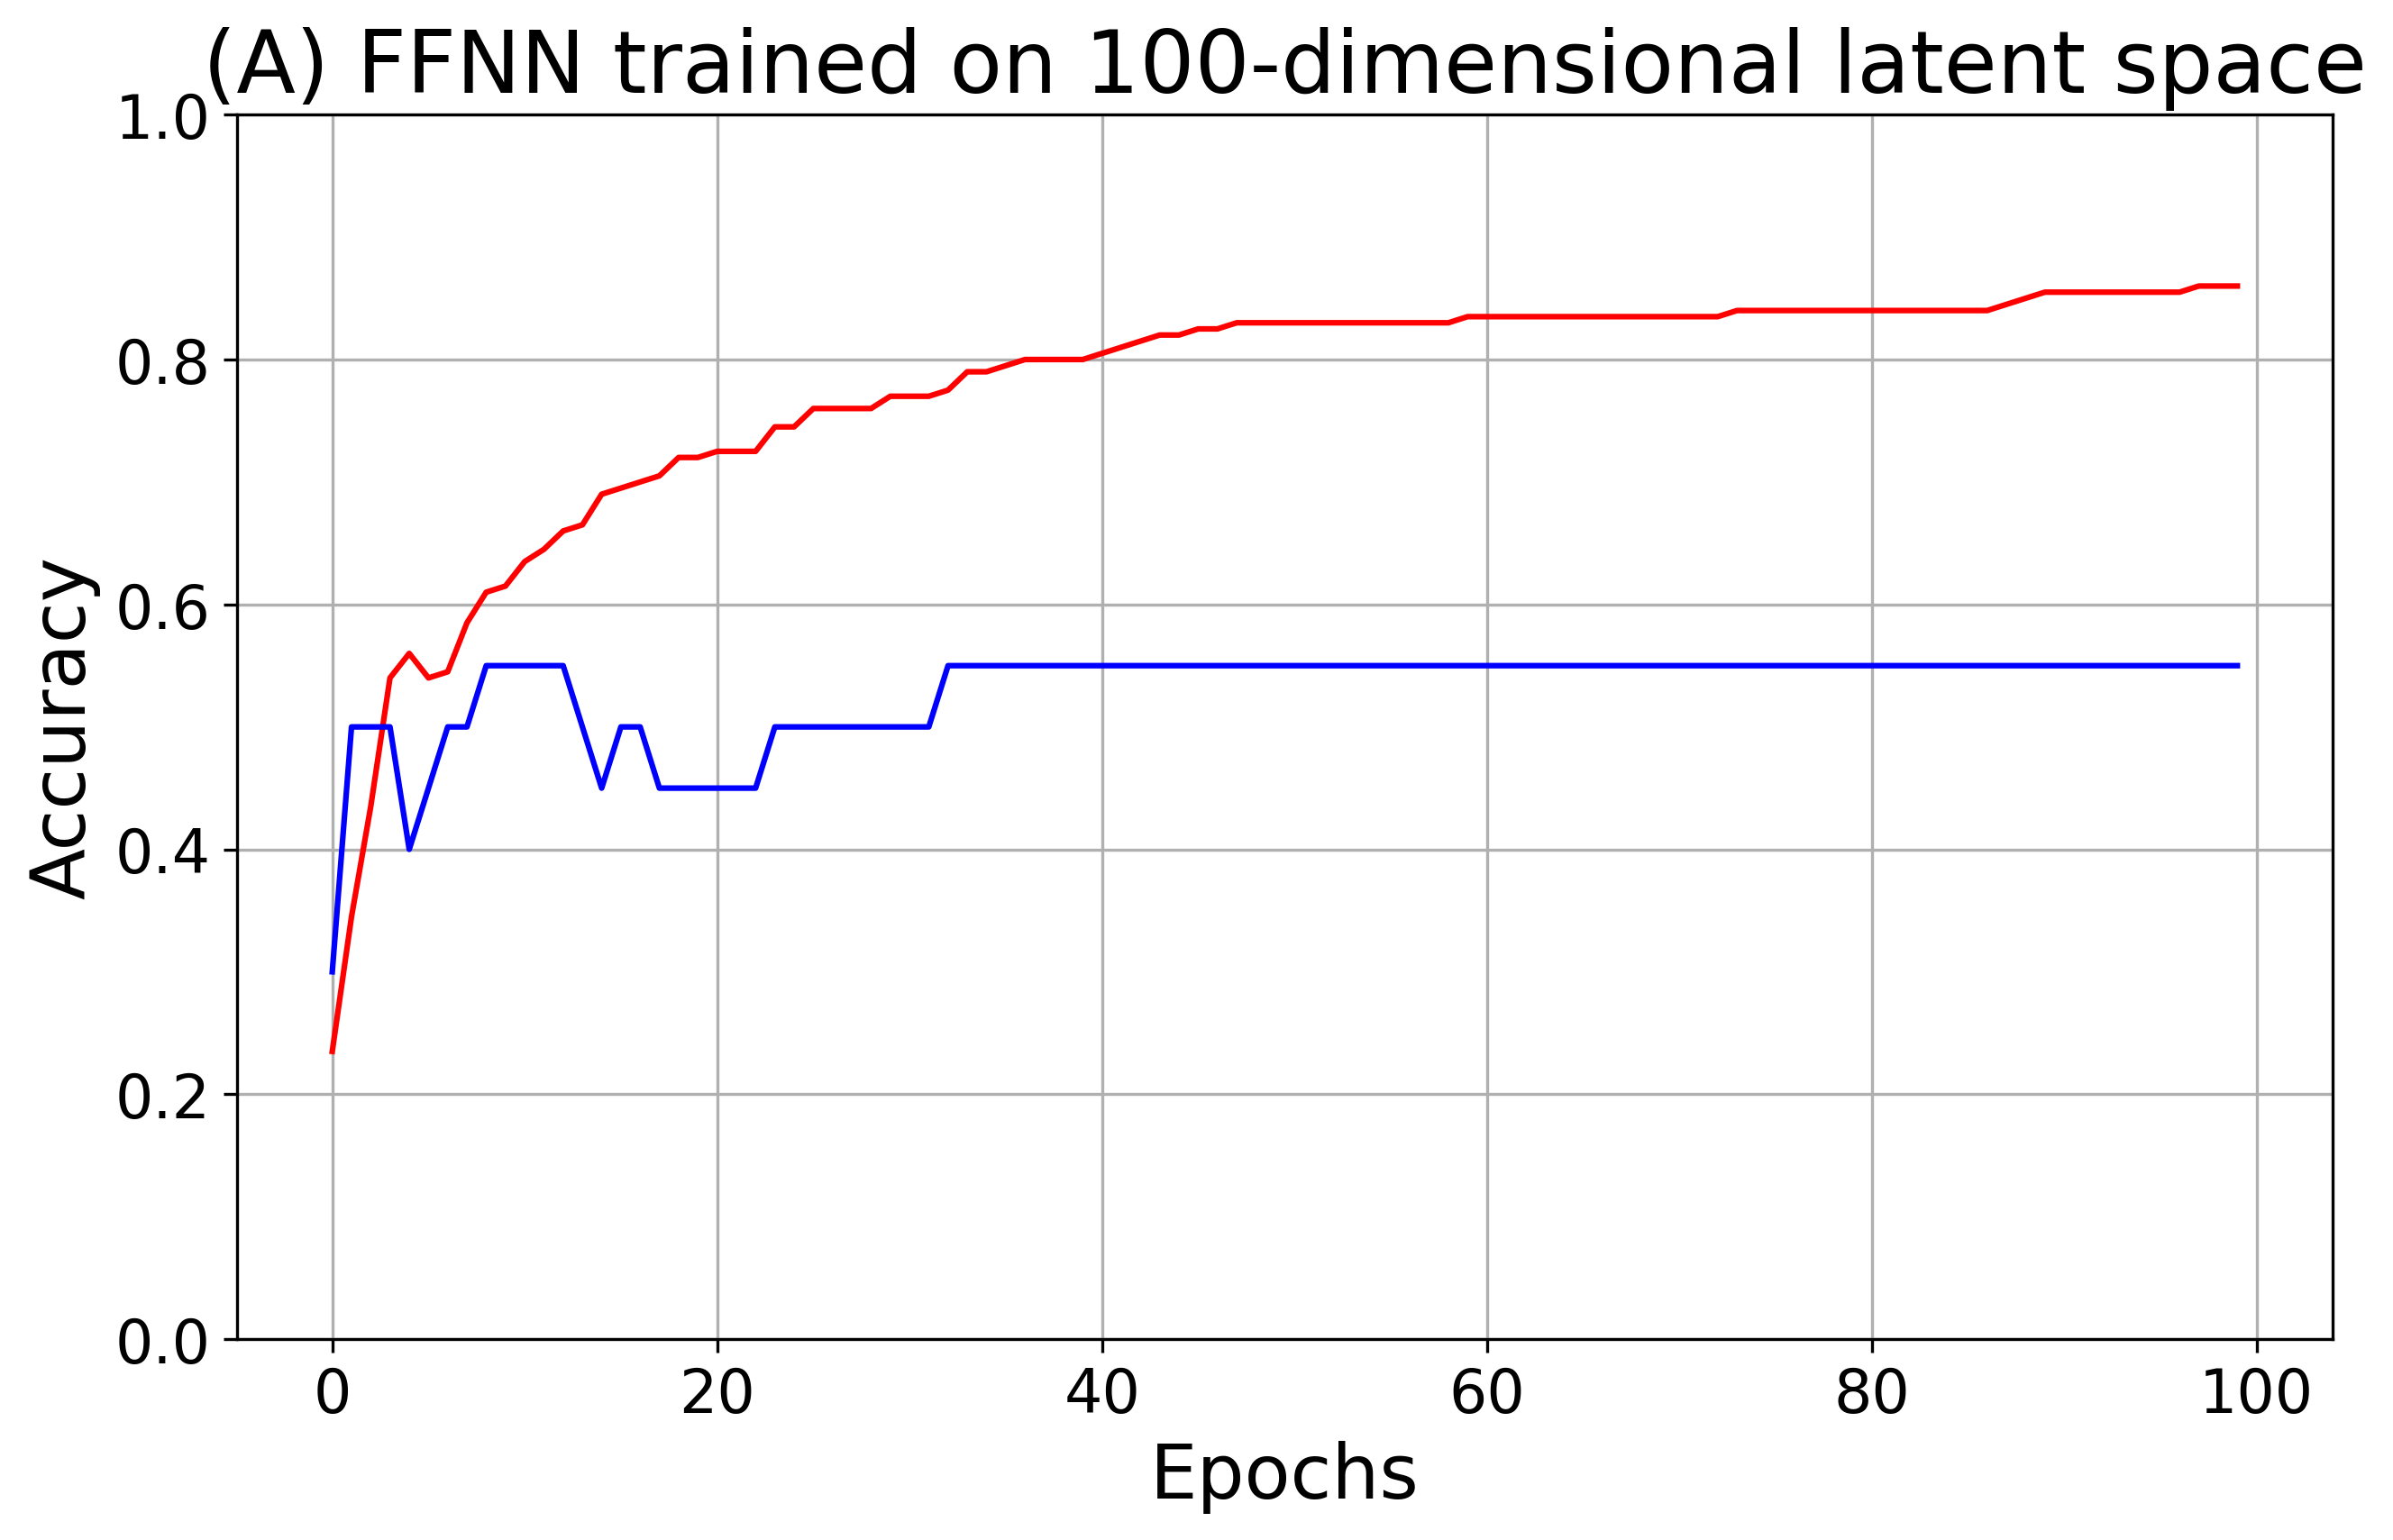
\includegraphics[width=0.99\textwidth]{latex poster/learning_curve.png}
\vspace{0.5cm}
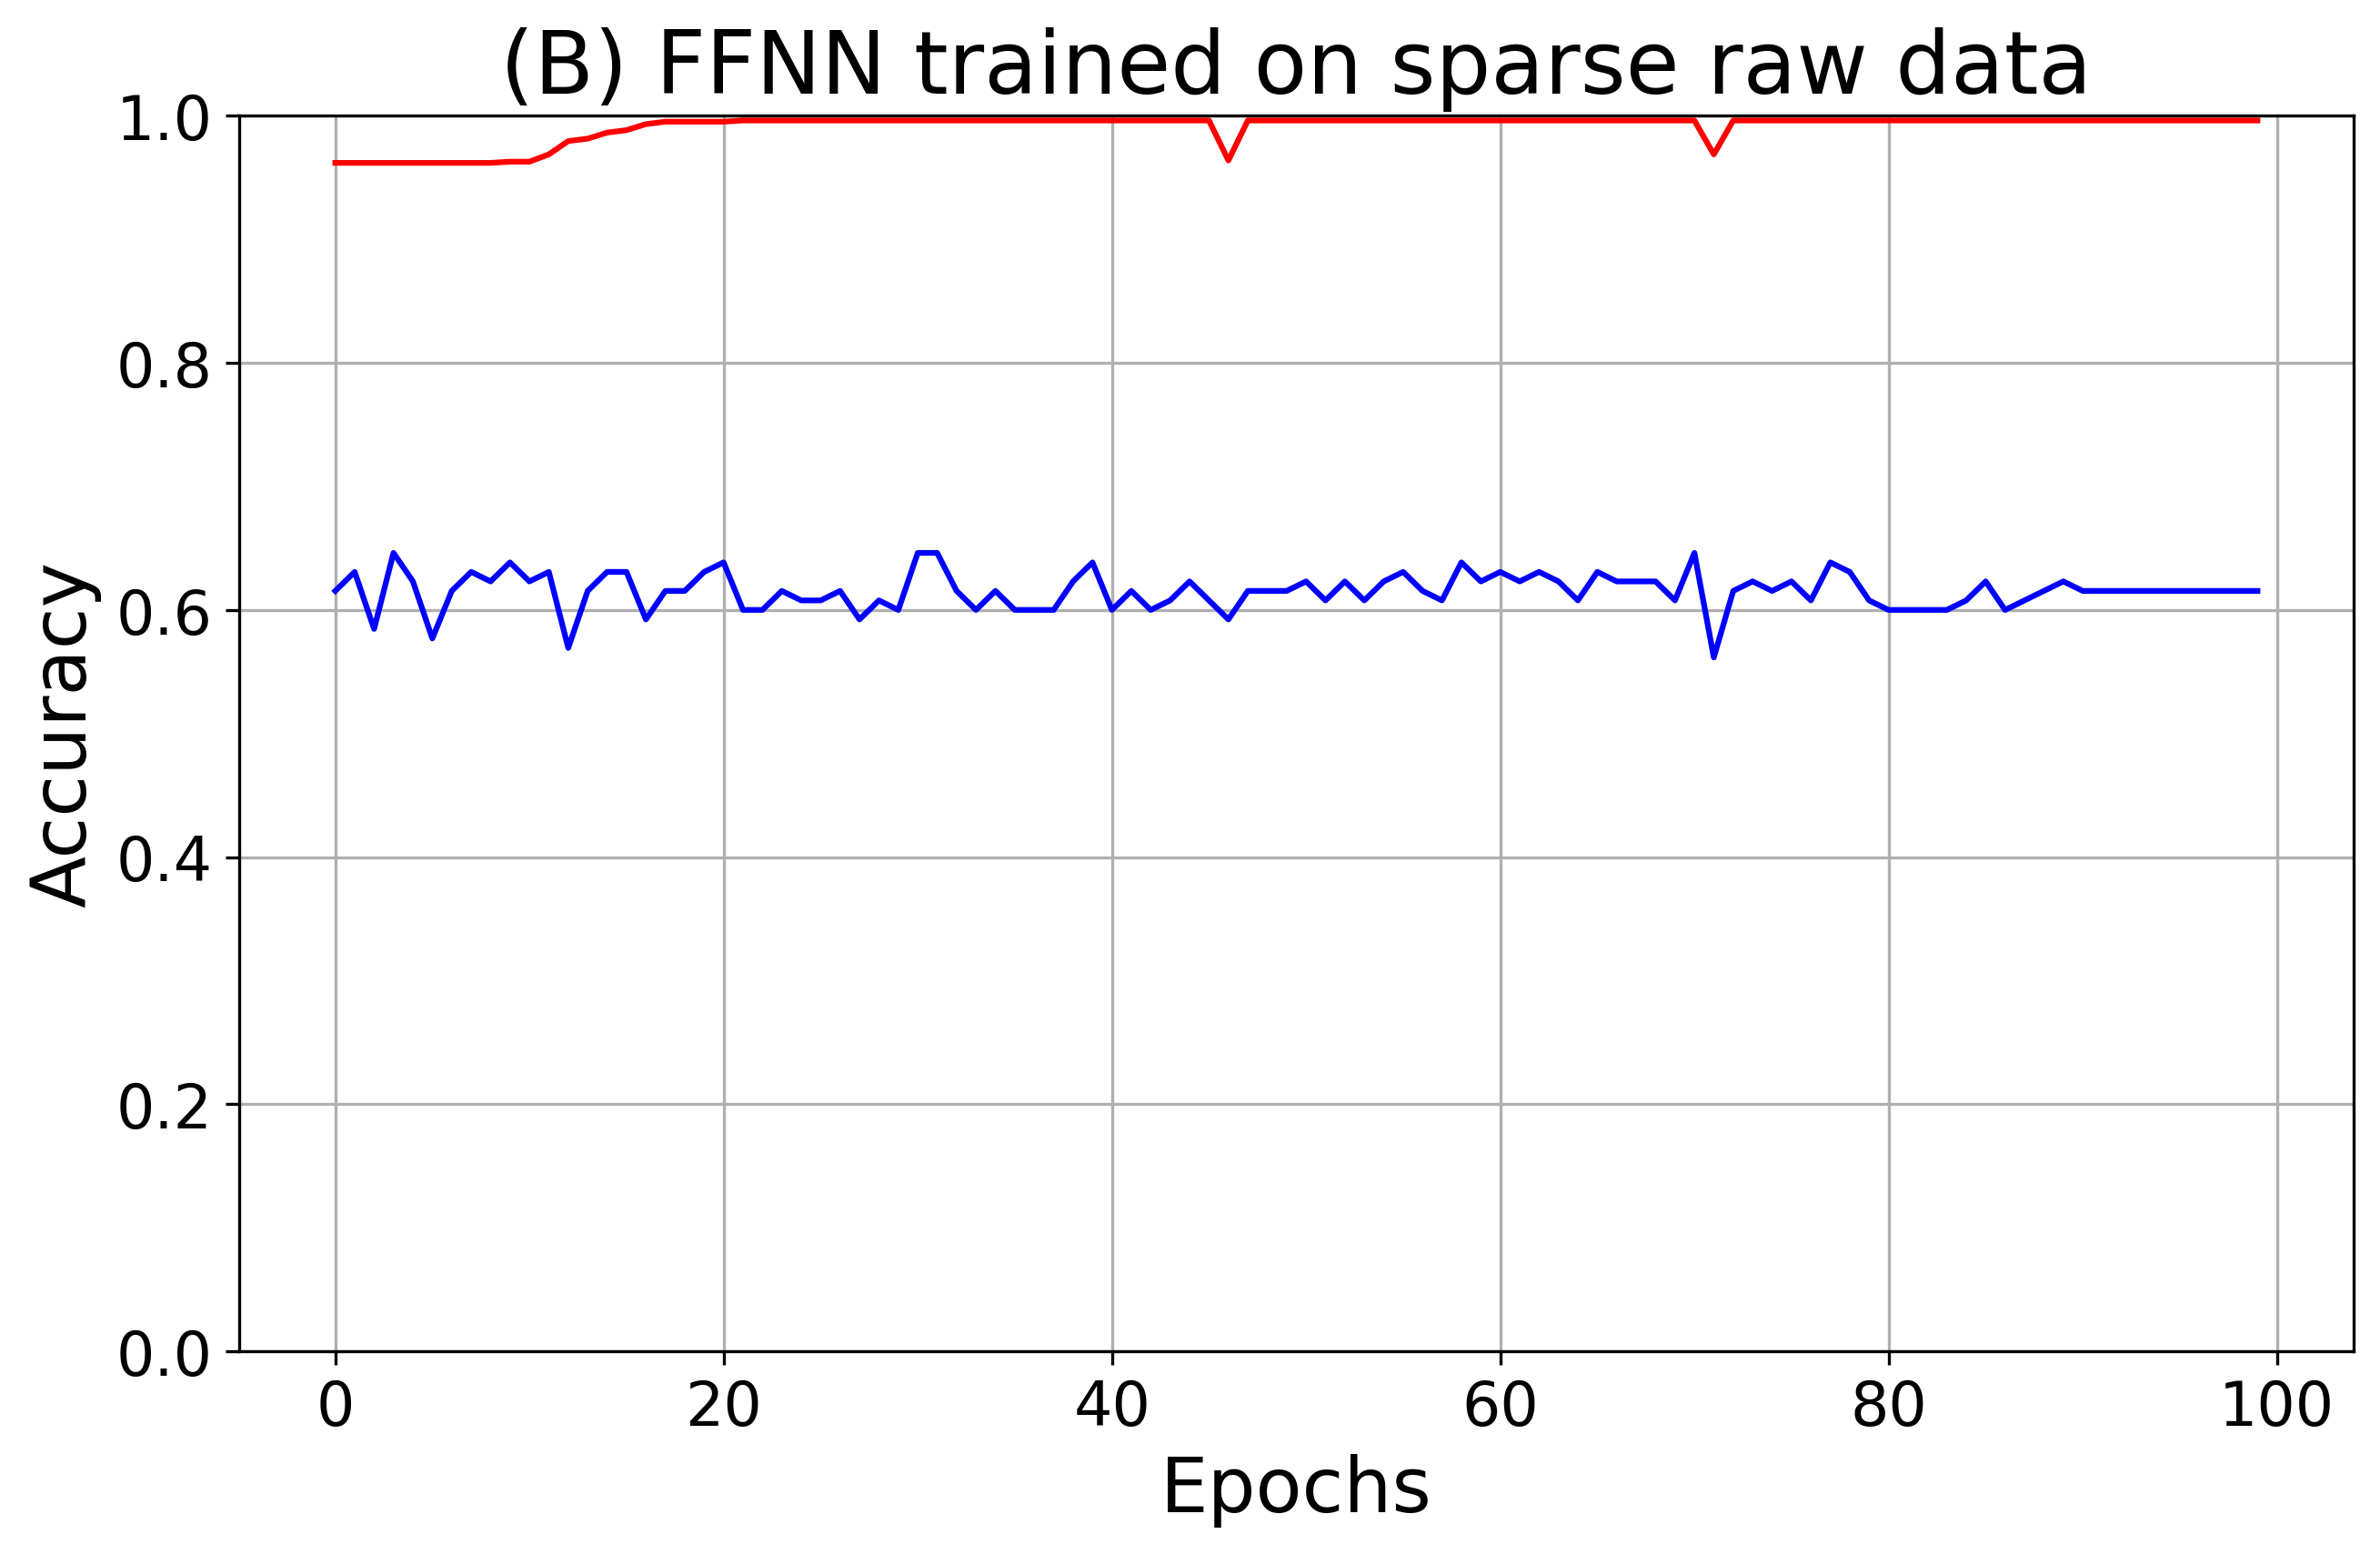
\includegraphics[width=0.99\textwidth]{latex poster/learning_curve (3).png}
\vspace{0.5cm}
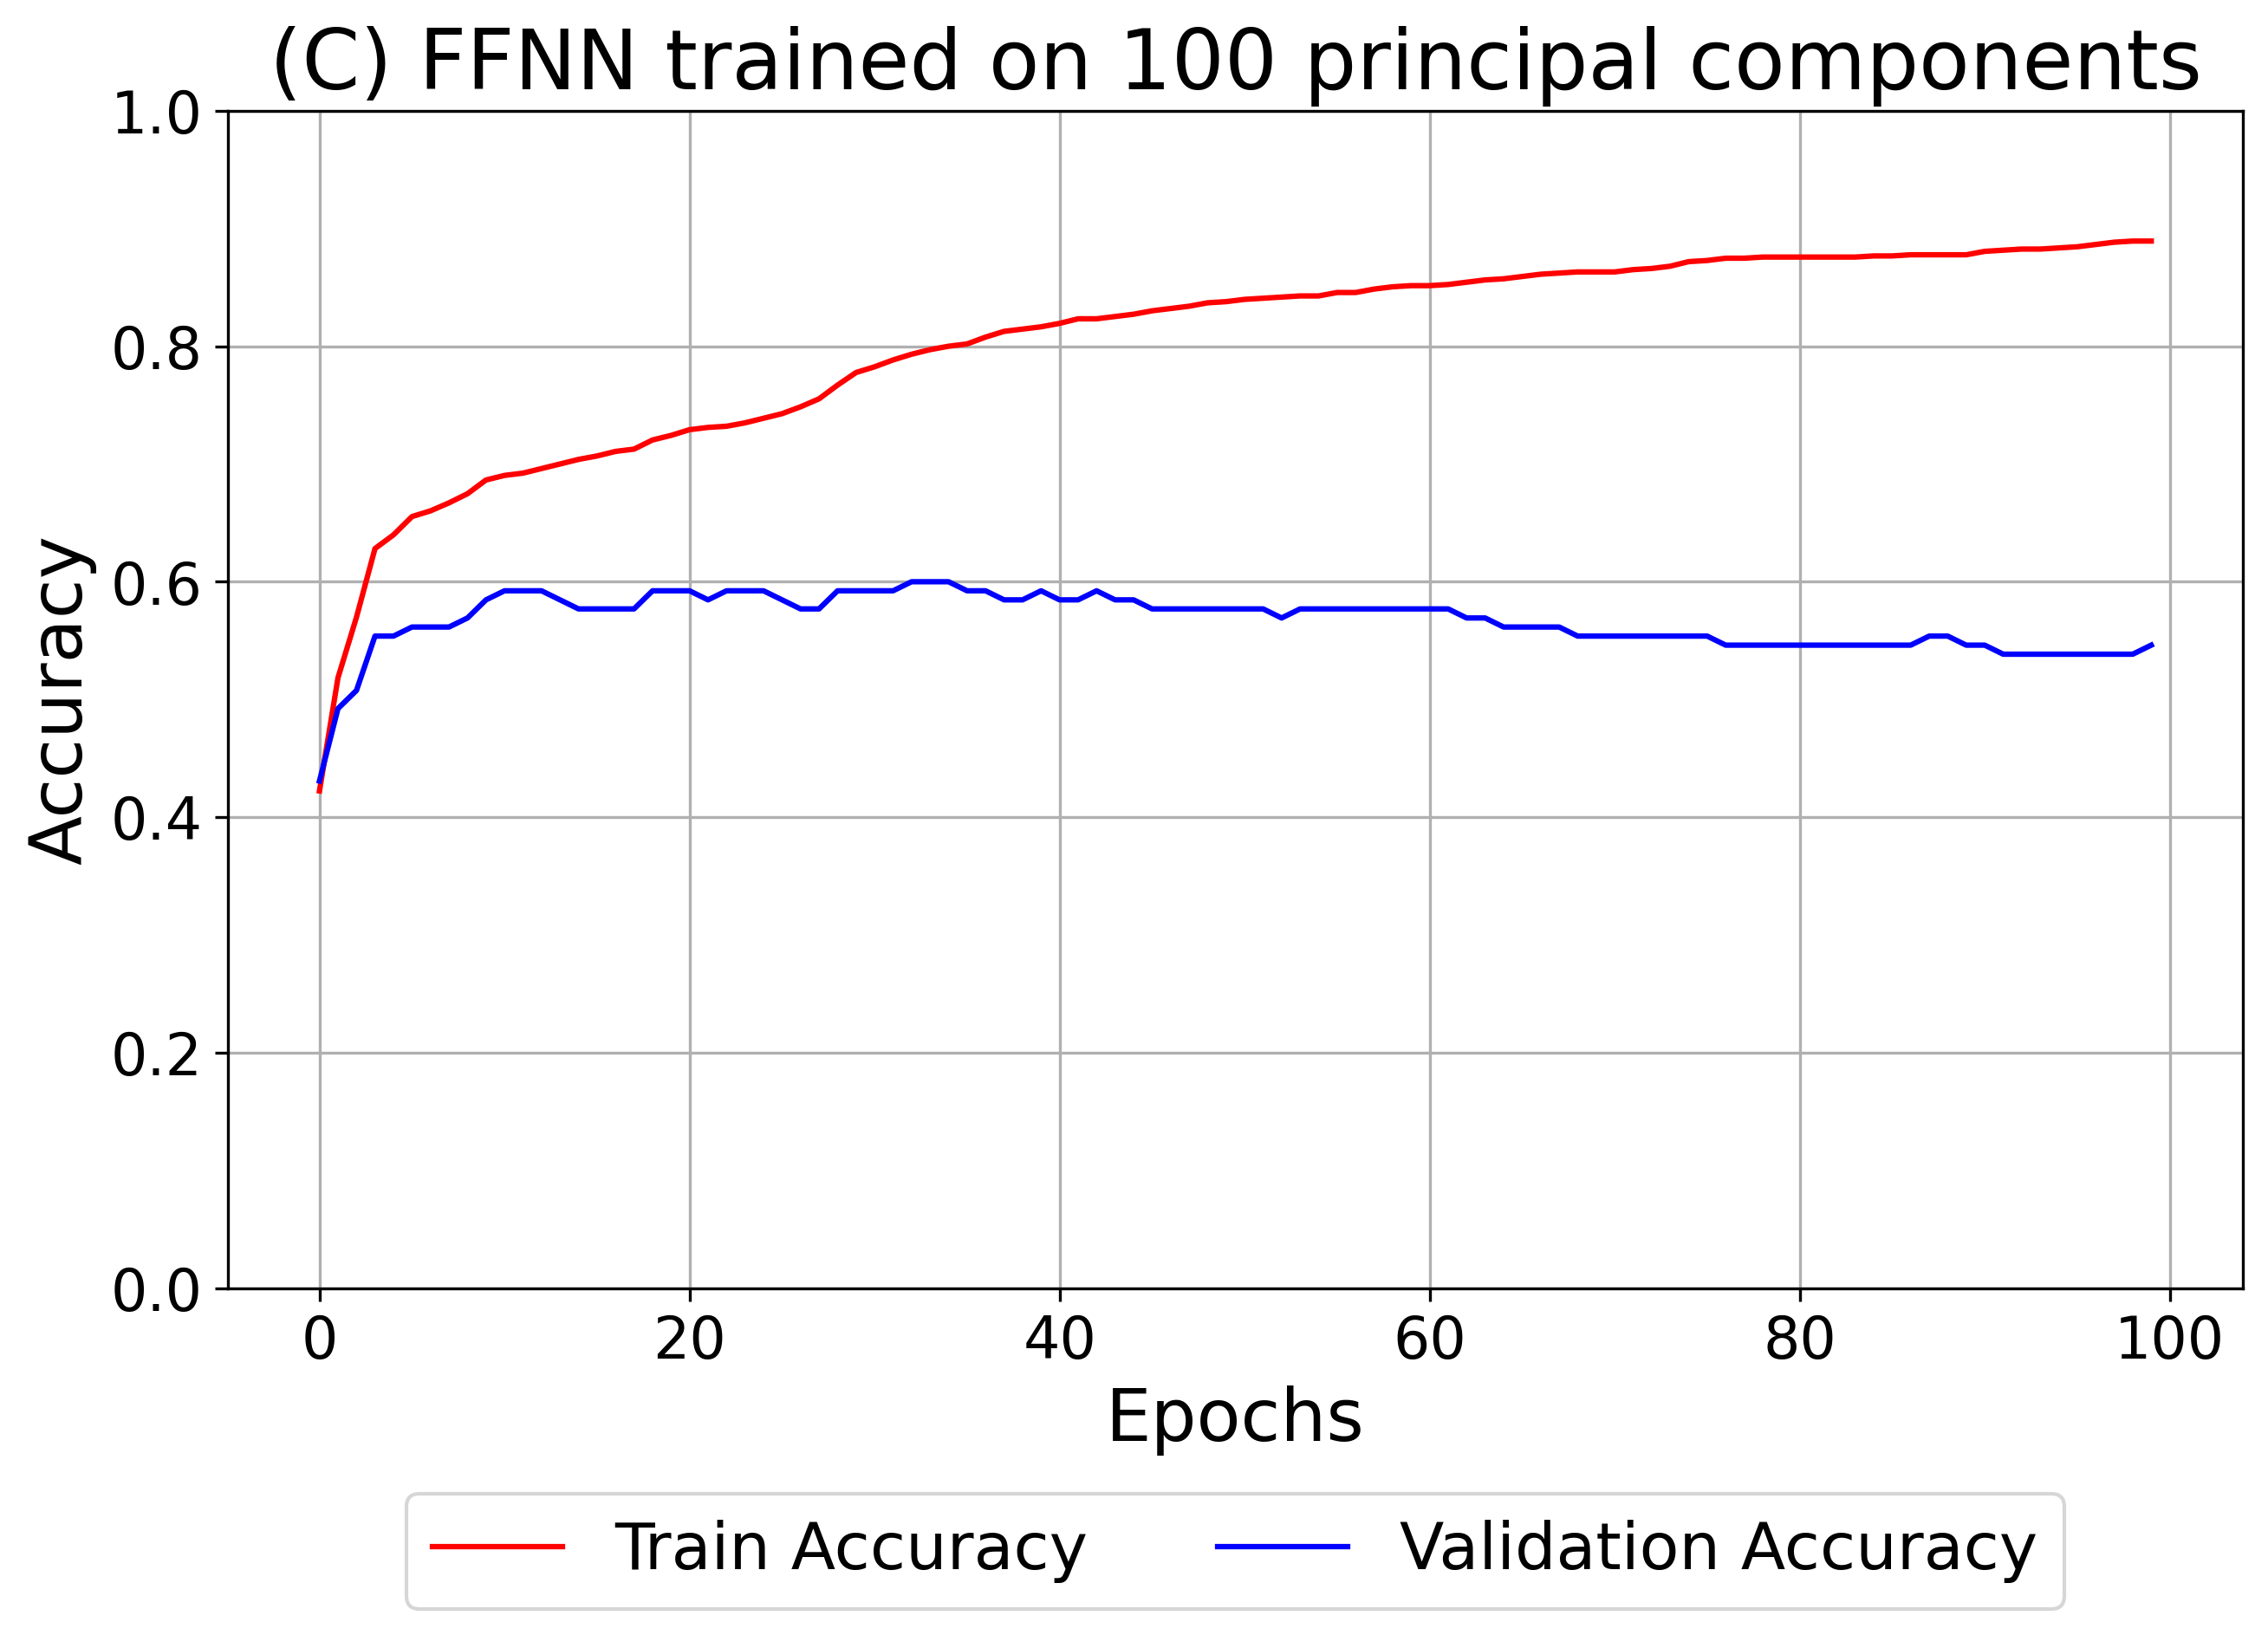
\includegraphics[width=0.99\textwidth]{latex poster/pca_learning_curve.png}
 \caption{Learning curves of FFNN trained with (A) scVAE latent representation (Z=100, H=500) (B) raw data (C) PCA (k=100)}
 \label{figure:training}
\end{figure}  

\end{minipage}

\end{column}
% -- COL 2
\begin{column}{0.49\textwidth}
\centering
%\vspace{2.5cm}
\centering
\begin{minipage}[t]{.95\textwidth}


\begin{figure}
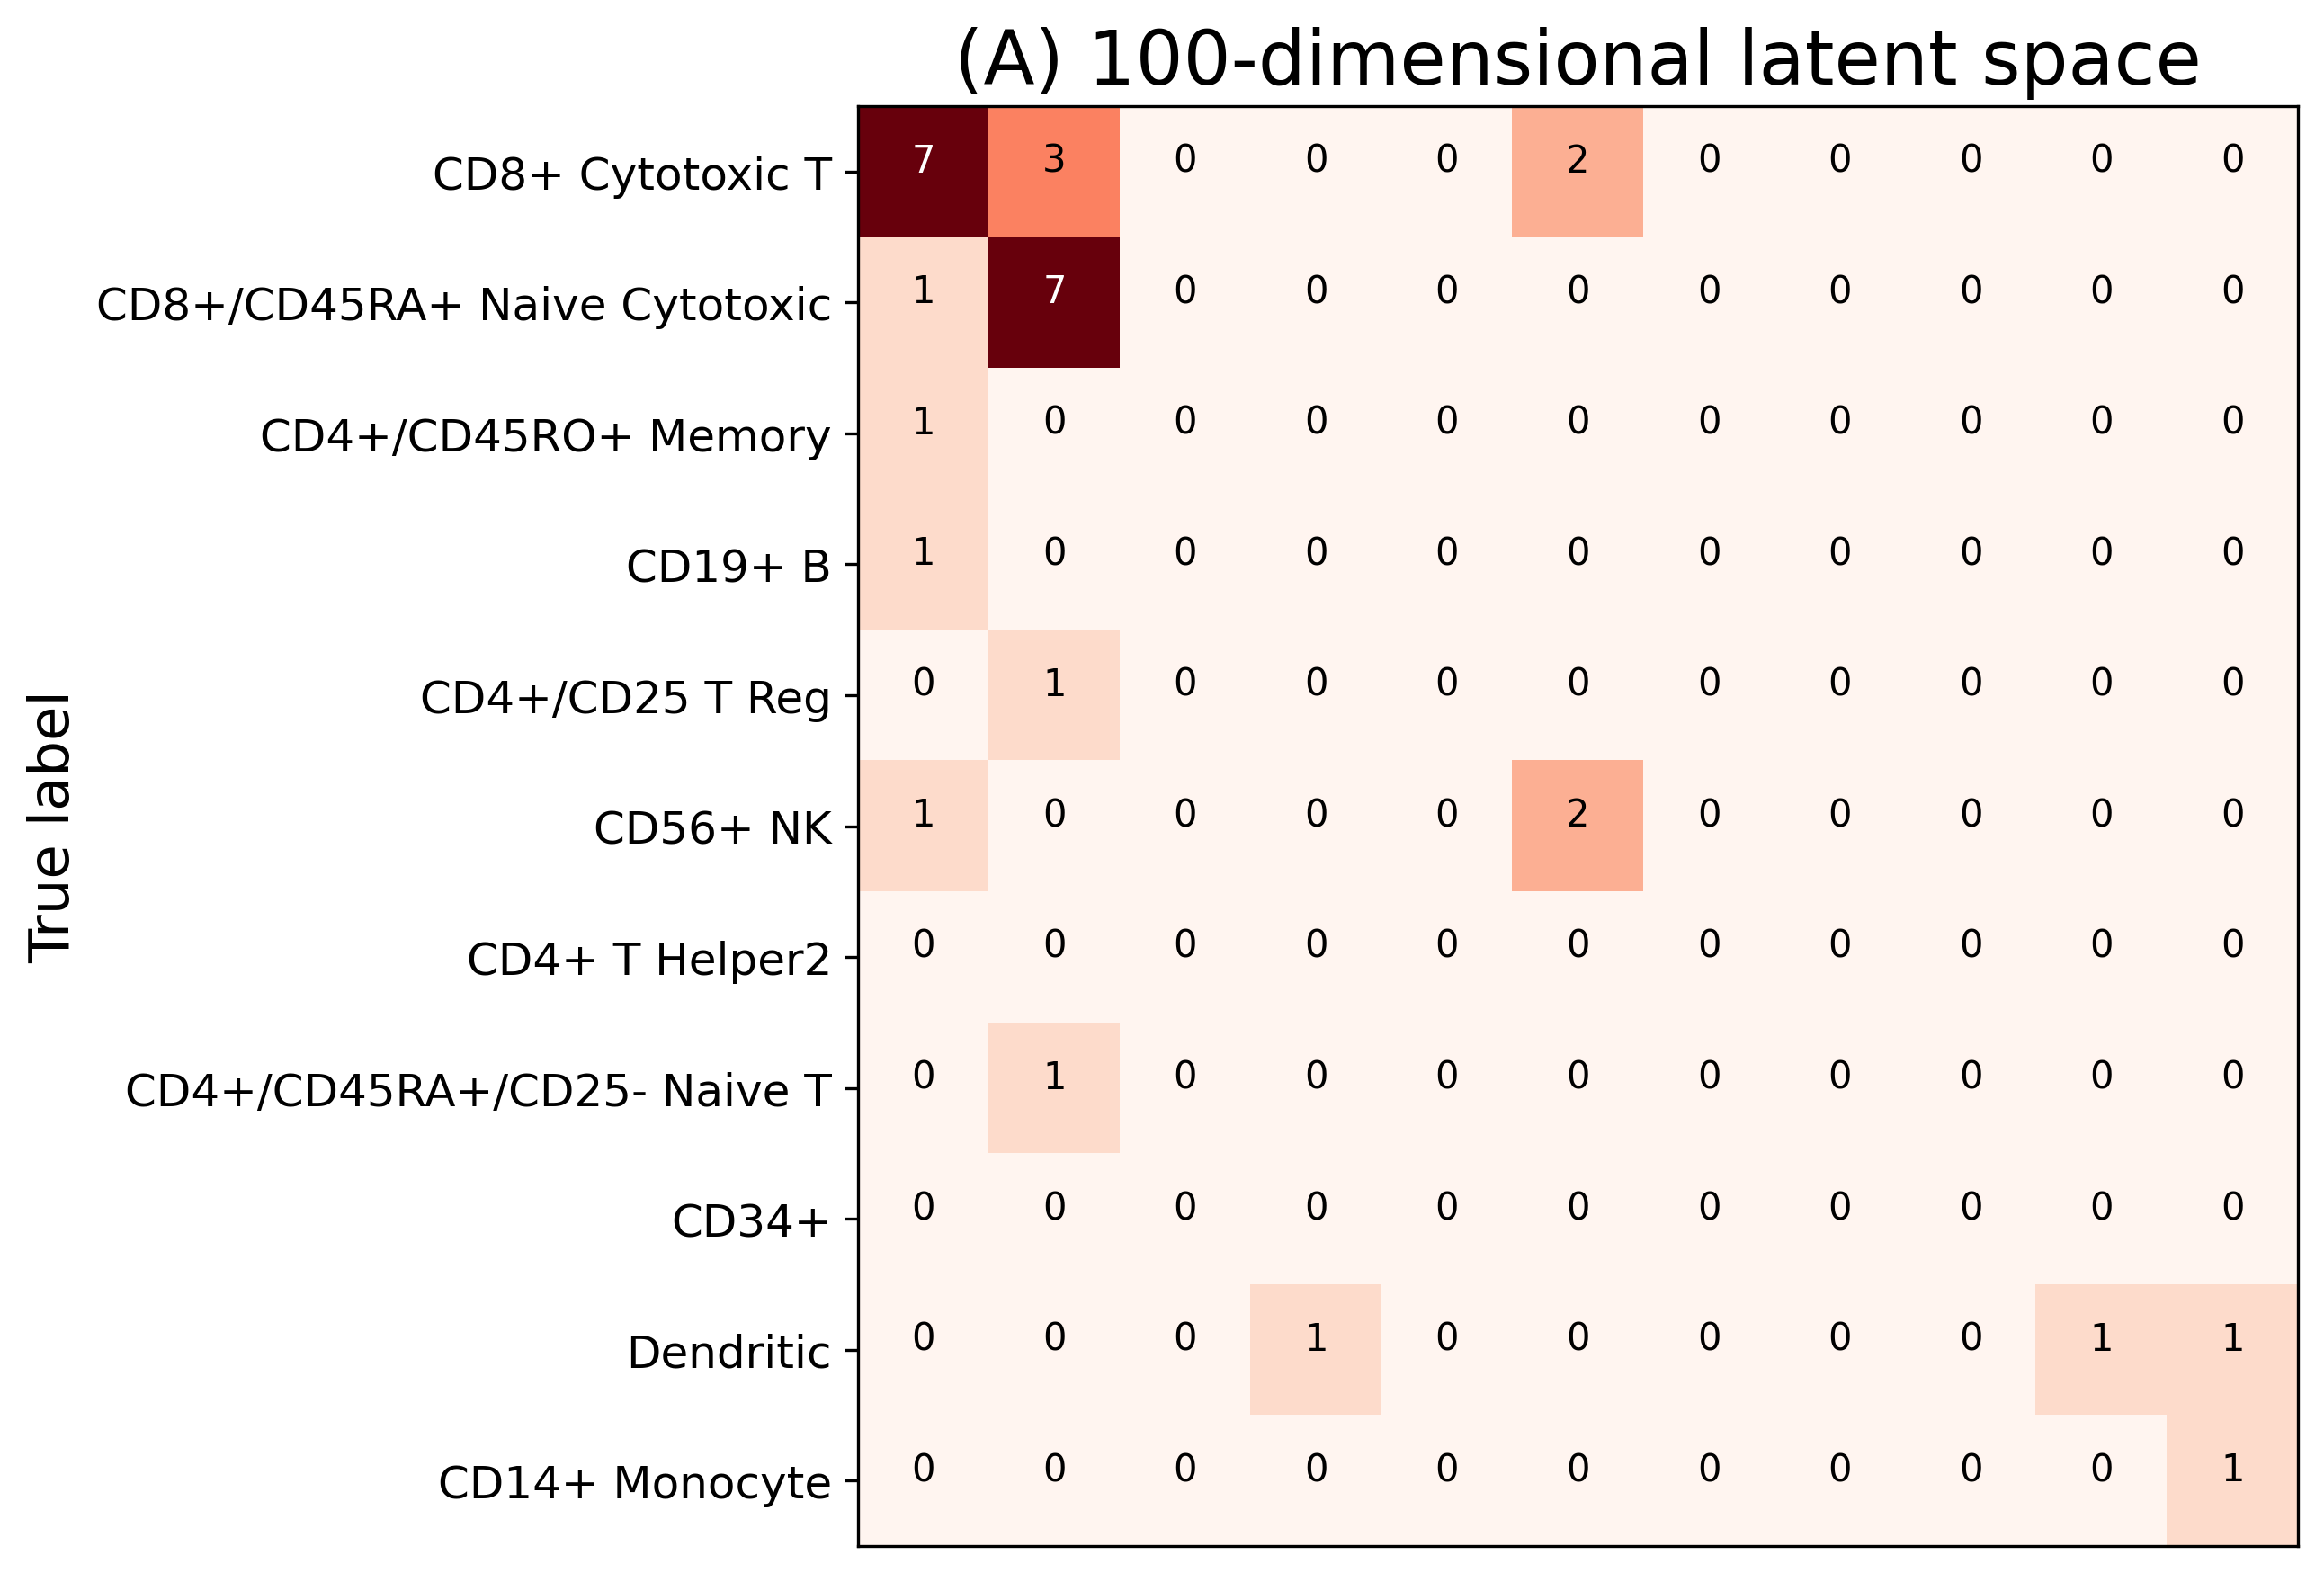
\includegraphics[width=1\textwidth]{latex poster/confusion (1).png}
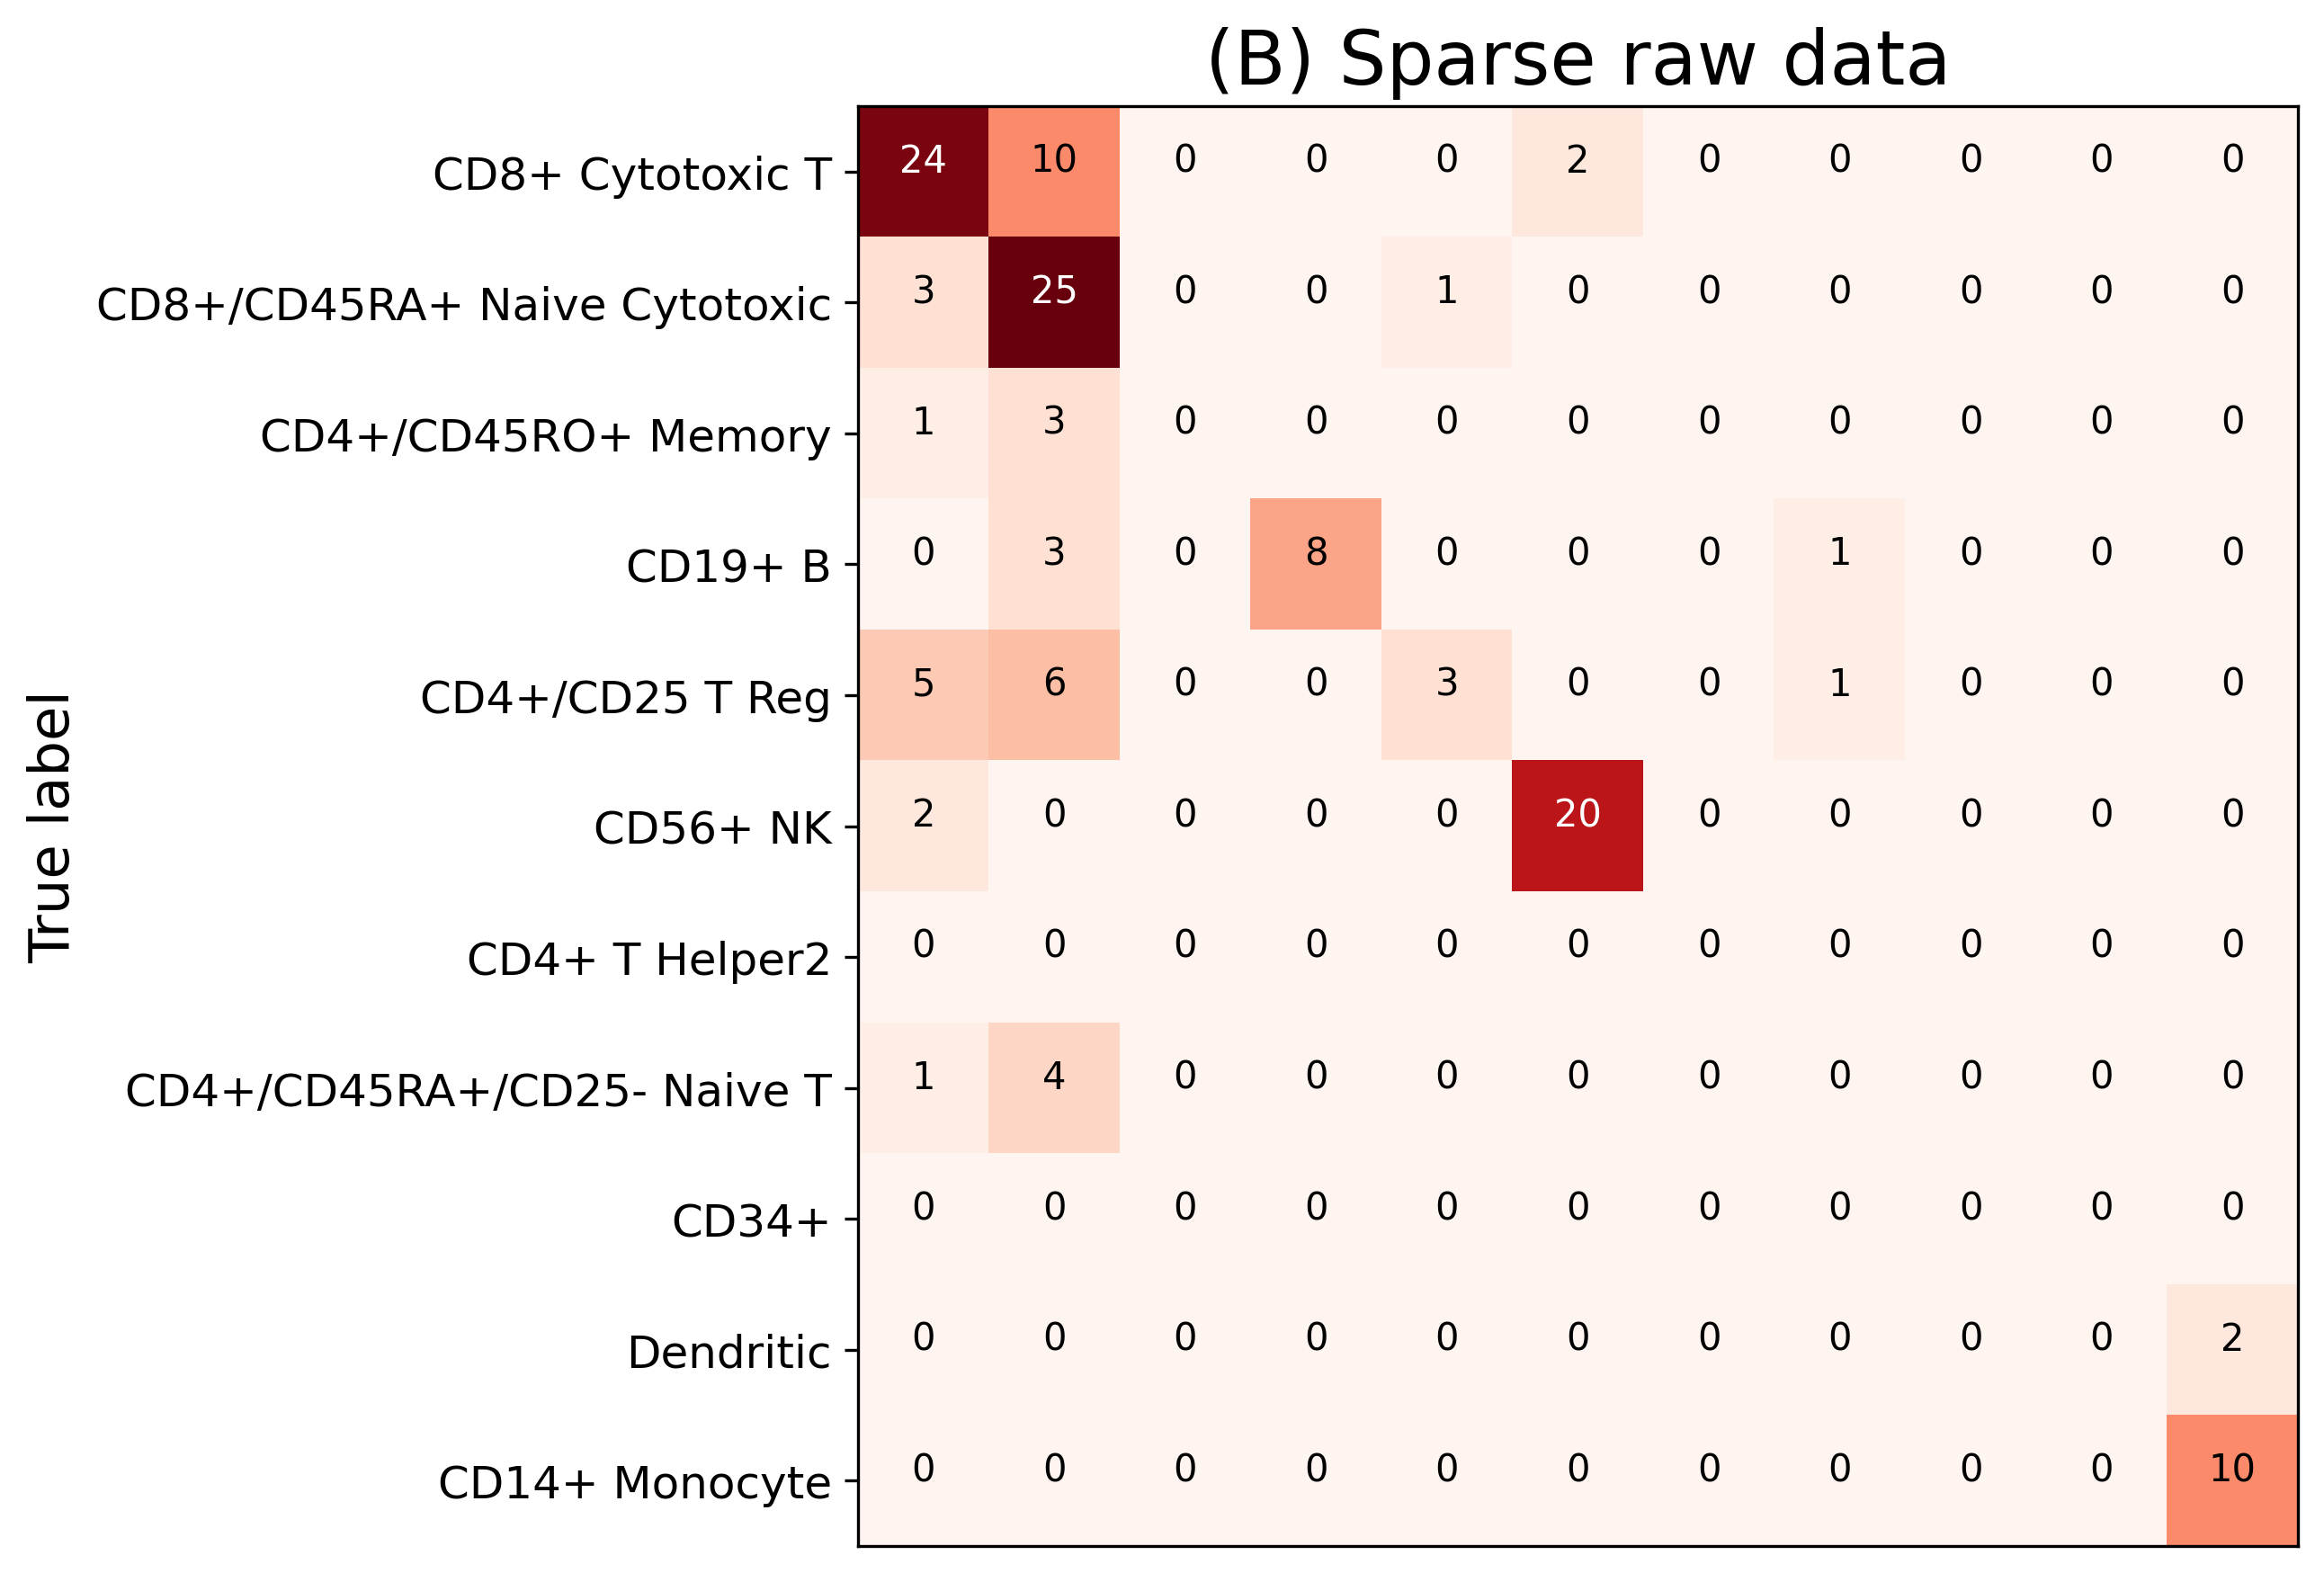
\includegraphics[width=1\textwidth]{latex poster/raw_confusion (1).png}
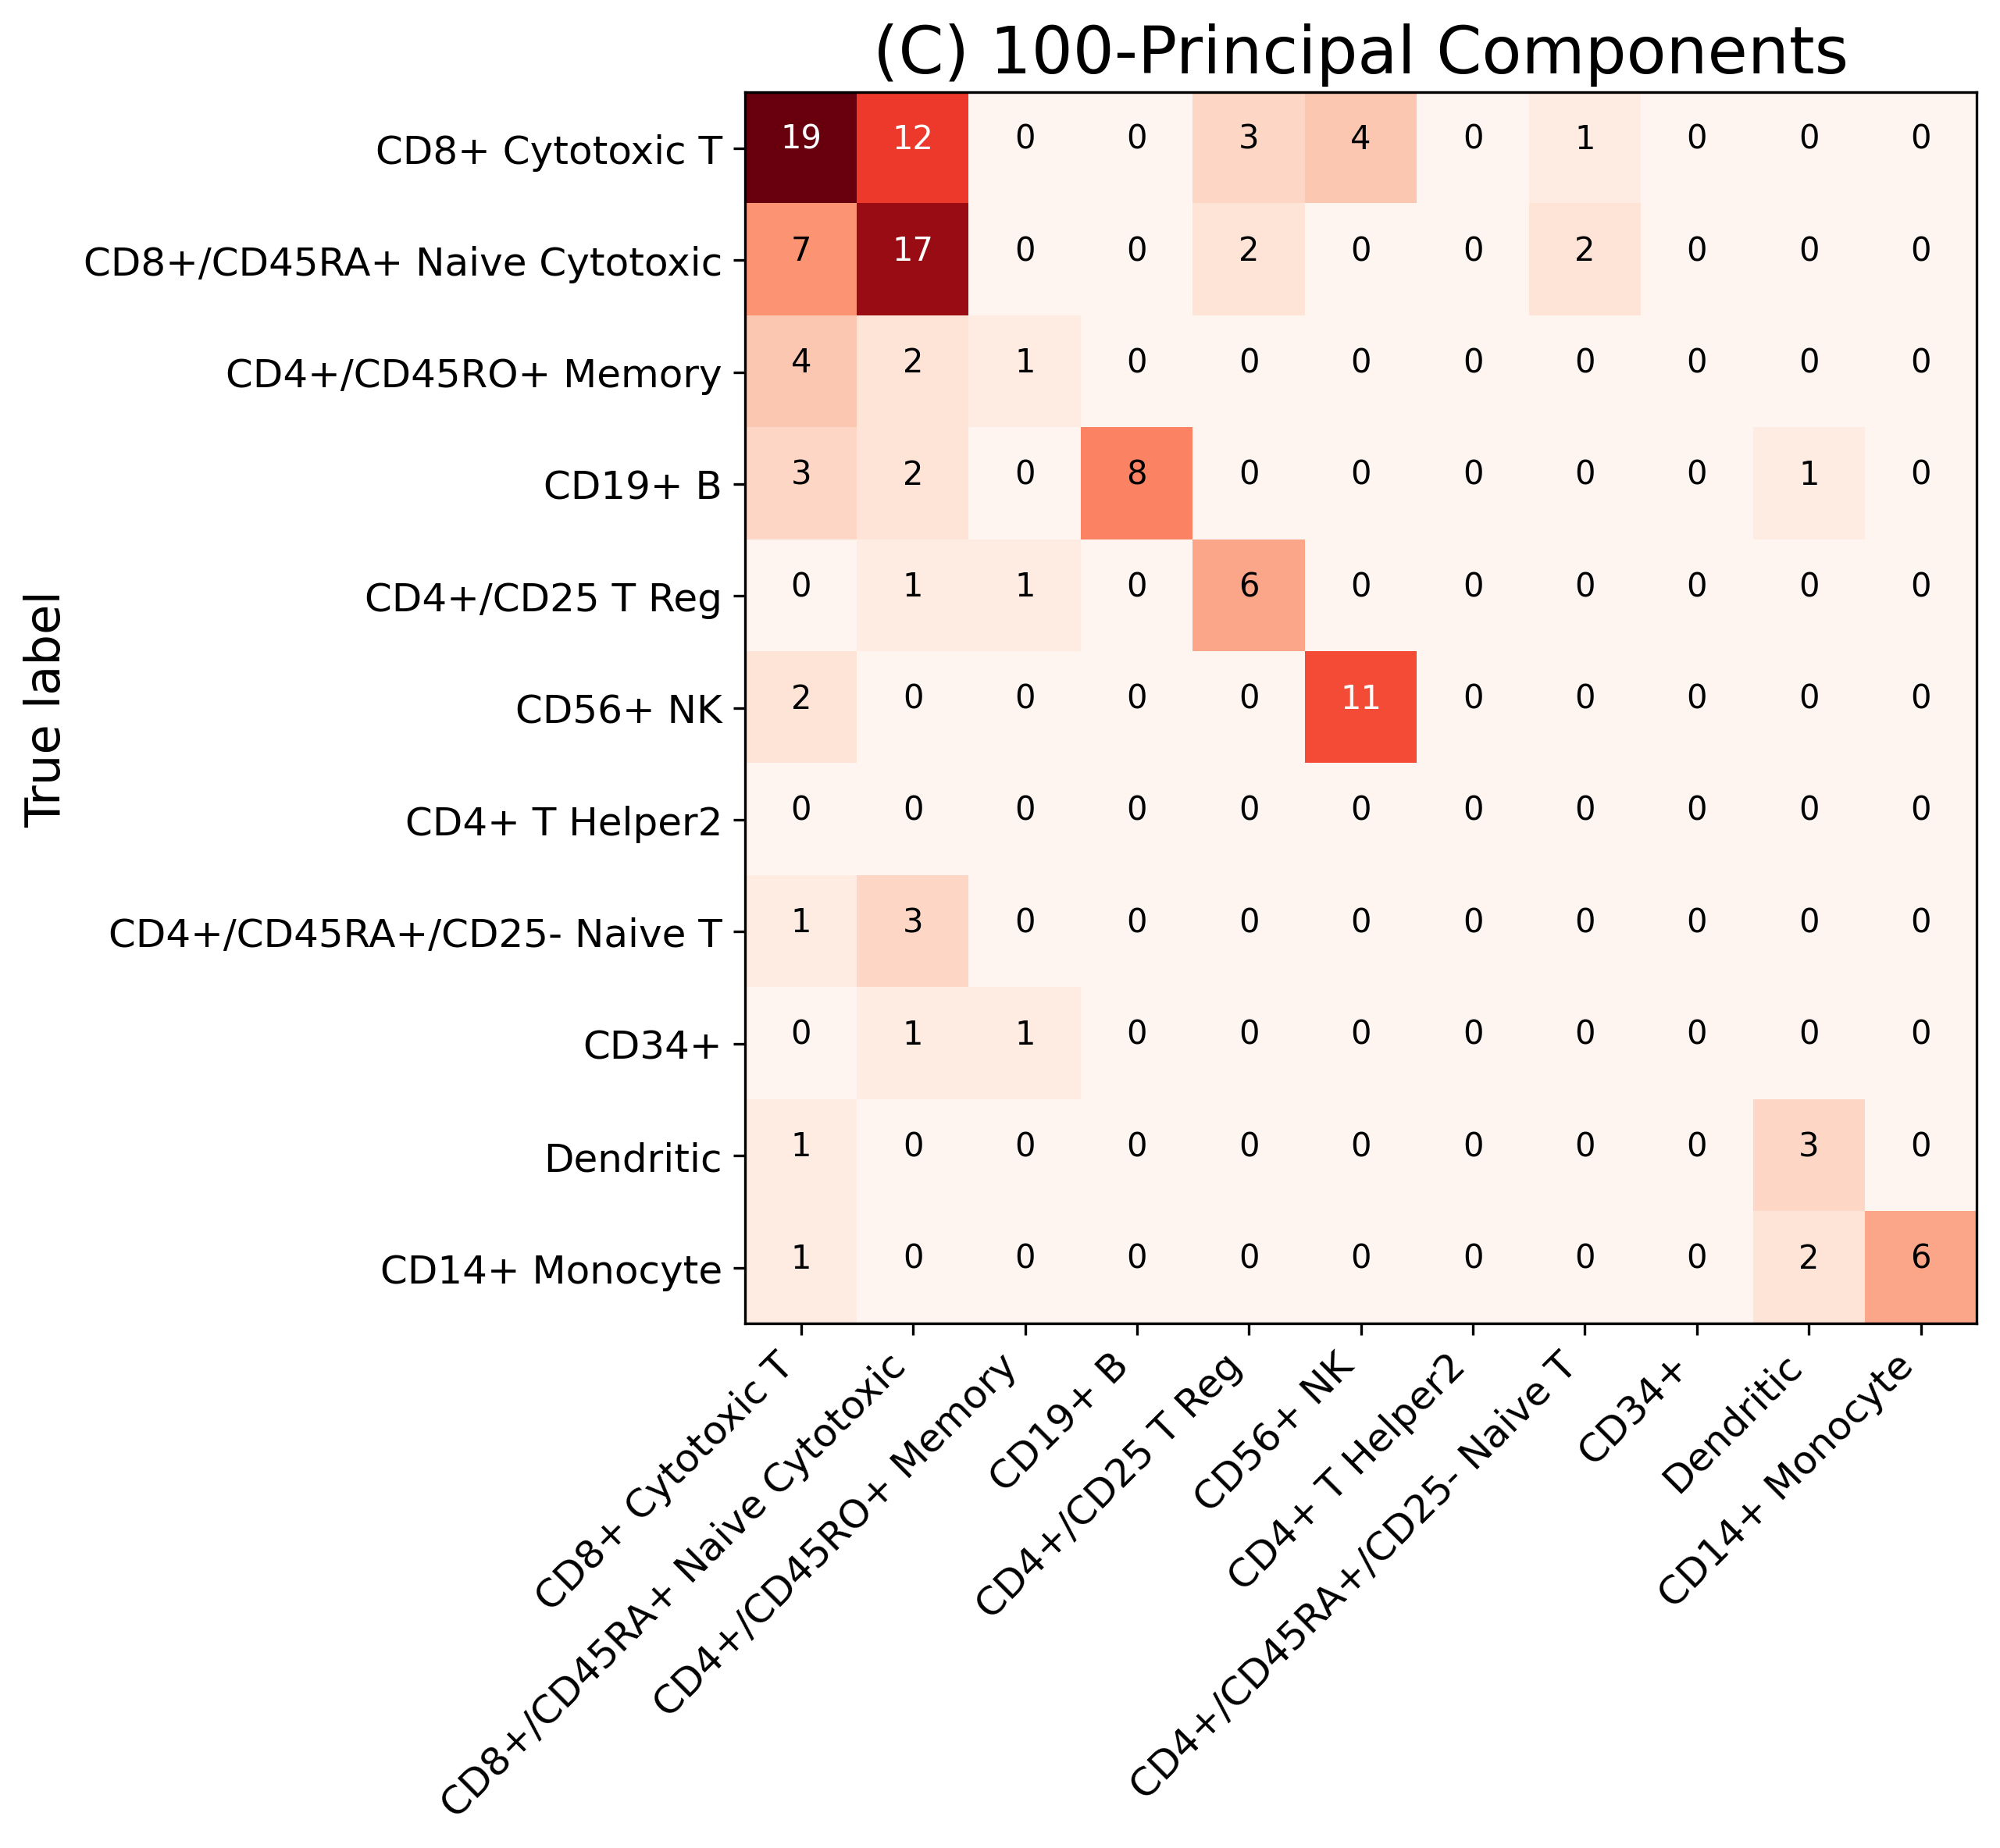
\includegraphics[width=1\textwidth]{latex poster/pca_confusion.png}
 \caption{Confusion matrices computed with test set from (A) scVAE latent representation (Z=100, H=500) (B) raw data (C) PCA (k=100)}
 \label{figure:confusion}
\end{figure}  
\end{minipage}
\end{column}
\end{columns}
\end{block}

\vfill

% ------------ new block -----
\begin{block}{Effect of dimensionality}

\begin{columns}
\begin{column}{0.40\textwidth}
\centering
\begin{minipage}[t]{.90\textwidth}

%\vspace{0.3cm}
\small{To evaluate the use of latent 
representations to classify cell types.
An FFNN was computed using latent representations with different dimensions.\\}
  

\end{minipage}
\end{column}

\begin{column}{0.60\textwidth}
\begin{minipage}[t]{.95\textwidth}
\centering
\begin{figure}
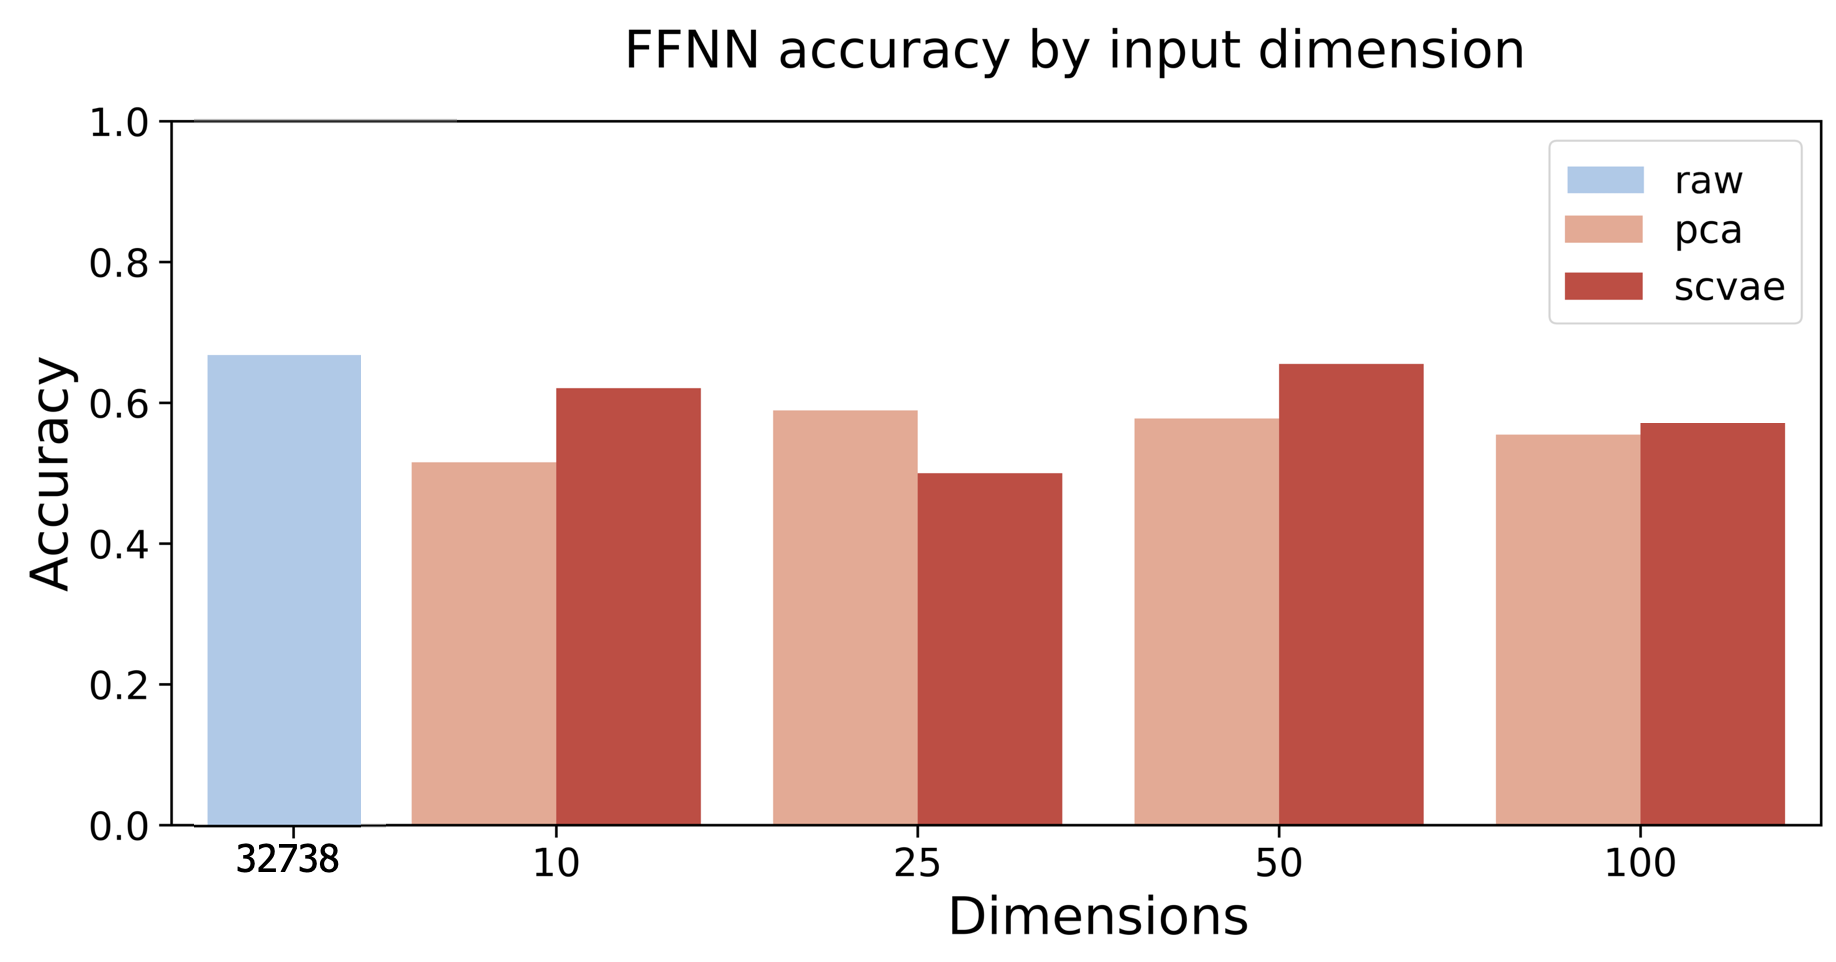
\includegraphics[clip,width=1\textwidth]{latex poster/dim_FFNN.png}
 \caption{Classification accuracy using input raw data, m PCA components and m dimensional latent space.}
 \end{figure} 
\end{minipage}
\end{column}
\end{columns}
\vspace{0.4cm}
\end{block}	
\vfill


% ------------ new block -----
\begin{block}{Conclusions}

\begin{columns}
\begin{column}{1\textwidth}
\begin{minipage}[t]{.95\textwidth}

\vspace{0.8cm}

\begin{itemize}
    \item \small{\textbf{scVAE} model performance was low in terms of  Rand Index and ELBO.}
    \vspace{0.3cm}
    \item \small{ Overfitting and no differences across inputs were observed in the \textbf{FFNN}.}
    \vspace{0.3cm}
    \item \small{These results could be explained by the \textbf{data set size}.}
\end{itemize}

\vspace{0.8cm}
\end{minipage}

\end{column}
\end{columns}
%\vspace{0.5cm}
\end{block}	

\vfill
% ------------ new block -----
\begin{block}{Future perspectives}
\centering
\vspace{0.5cm}
\small{
\begin{itemize}
    \item \small{ Increase training \textbf{data set size} for training scVAE models. }
    \vspace{0.3cm}
    \item \small{ \textbf{Validate} current scVAE model on other external data sets.}
    \vspace{0.3cm}
    \item \small{Train scVAE on \textbf{different data sets}.}
\end{itemize}
}
\vspace{0.8cm}

\end{block}
\vfill
\begin{block}{References}

{\footnotesize
\bibliographystyle{abbrvnat}	
\bibliography{biblio}
}			
\end{block}
\vfill

         
}
\end{minipage}
\end{beamercolorbox}
\end{column}
\end{columns}
% ---------------------------------------------------------%
% end the COLUMN 2
% ---------------------------------------------------------%
 
\vskip1ex
%\tiny\hfill\textcolor{ta2gray}{Created with \LaTeX \texttt{beamerposter}  \url{http://www-i6.informatik.rwth-aachen.de/~dreuw/latexbeamerposter.php}}
\tiny\hfill{Created with \LaTeX \texttt{beamerposter}  \url{http://www-i6.informatik.rwth-aachen.de/~dreuw/latexbeamerposter.php} \hskip1em}
\end{frame}
\end{document}